\documentclass{beamer}
\usepackage{animate}
\usepackage{multimedia}
\usepackage{hyperref}
\usepackage{amsmath}
\usepackage[latin1]{inputenc}
\usetheme{CambridgeUS}

\title{Combined Adaptive Multimesh hp-FEM/hp-DG for Multiphysics Coupled Problems of Compressible Flow}
\author{\underline{Lukas Korous}, Milan Hanus, Pavel Solin} 
\institute{University of Nevada, Reno}

\begin{document}

\begin{frame}
\titlepage
\end{frame}

%Acknowledgement
\begin{frame}
We acknowledge the financial support by Subcontract No. 00089911 
of Battelle Energy Alliance (U.S. Department of Energy intermediary) 
\end{frame}

%Intro
\begin{frame}
\frametitle{Motivation}
In multiphysics problems, physical field exhibit qualitative differences:\\
\begin{itemize}
\item singularities
\item boundary layers
\item smooth areas
\end{itemize}\ \\
These phenomena require specific treatment.\\\ \\
Our goal: approximate every physical quantity in an optimal way.\\
\begin{itemize}
	\item appropriate mesh (for each component of the system)
\item appropriate Sobolev space ($H^1, L^2, H_{curl}, H_{div}$, ..)
\item appropriate method (continuous FEM, DG method) of higher order
\end{itemize}
\end{frame}

%Multimesh example
%different quantities can be approximated using different meshes\\\ \\
%difference in number, size, and distribution of elements\\\ \\
%difference in orders of the polynomials used for approximation on each element\\
\begin{frame}
 \frametitle{Component specific meshes example}
	Coupled system of linear second-order PDE\\
	Heat and moisture transfer in concrete.
$$\movie[height=0.6\textheight]{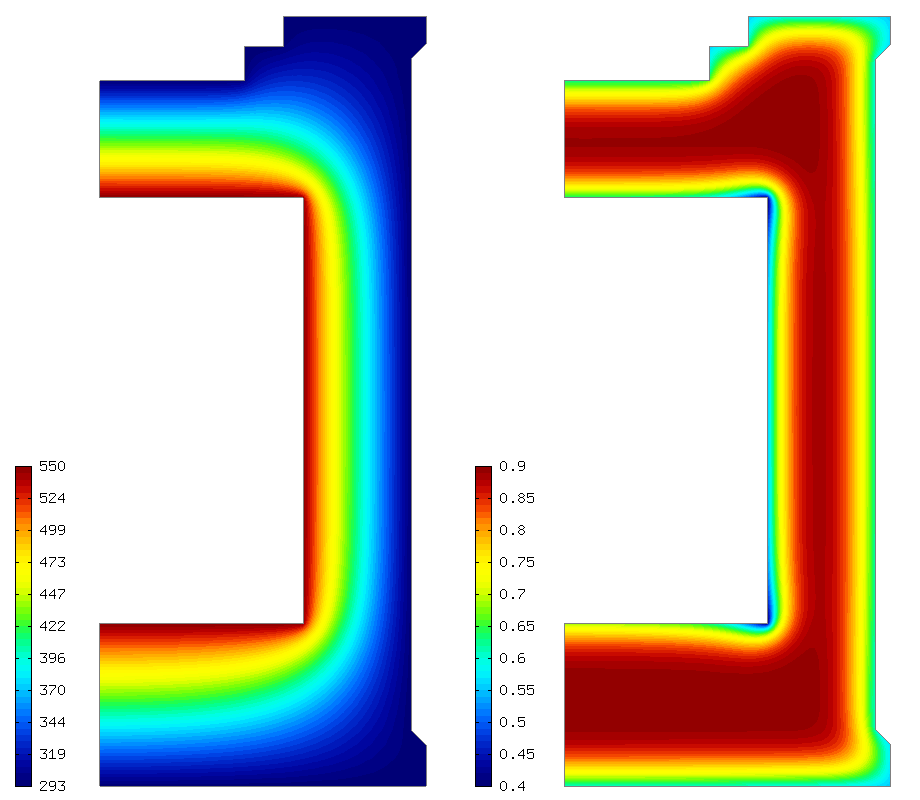
\includegraphics[height=0.6\textheight]{hm-sln-frame.png}}{hm-sln.avi}$$
\end{frame}

\begin{frame}
 \frametitle{Component specific meshes example}
	Coupled system of linear second-order PDE\\
	Heat and moisture transfer in concrete.
$$\movie[height=0.6\textheight]{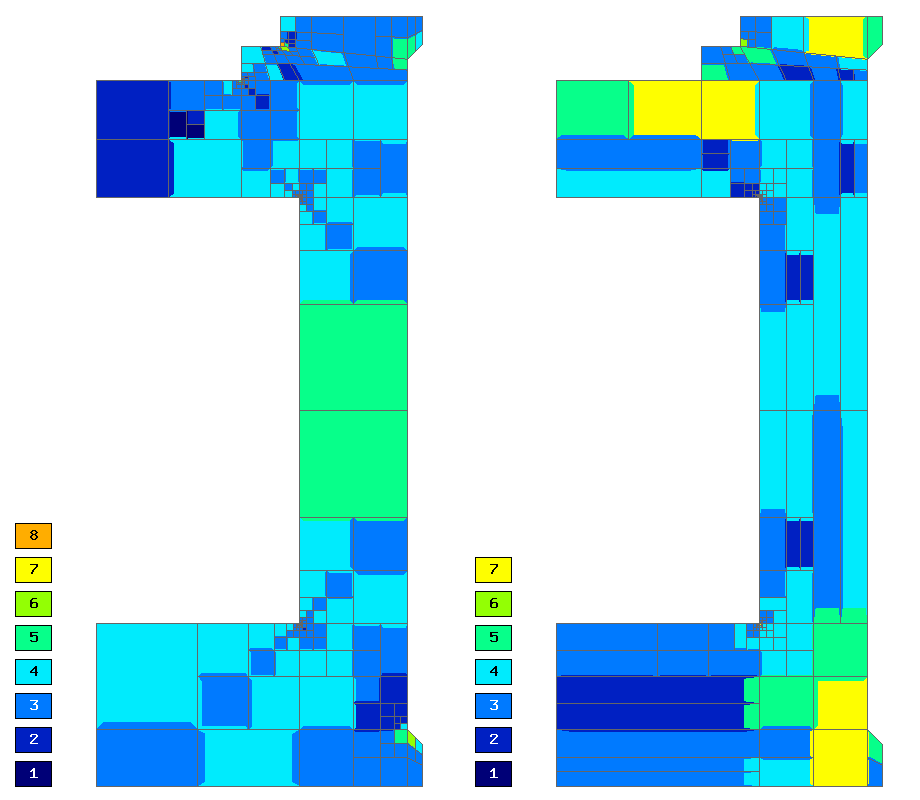
\includegraphics[height=0.6\textheight]{hm-mesh-frame.png}}{hm-mesh.avi}$$
\end{frame}


%Multimesh example - DOFs
\begin{frame}
\frametitle{Component specific meshes example - DOFs}
\begin{center}
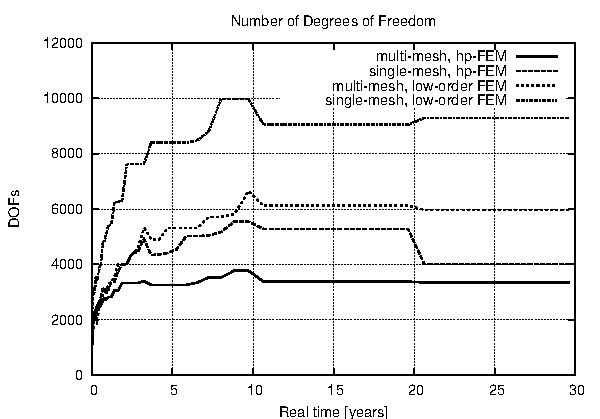
\includegraphics[width=0.8\textwidth]{reactordofscompare.pdf}
\end{center}
% Comparison of lower orders, higher orders, multimesh vs. non-multimesh
\end{frame}

%How multimesh works
\begin{frame}
\frametitle{Monolithic Multimesh Adaptive FEM}
\begin{itemize}
\item meshes come from one \textbf{common coarse mesh} (can be one element) that we call master mesh\\\ \\
\item every mesh in the system is obtained from this one via an \textbf{arbitrary sequence of} elementary \textbf{refinements}\\\ \\
\item adaptivity puts all elements of all meshes into one array, error estimate as a difference between the coarse and reference mesh approximations\\ \ \\
\item elements sorted according to the error, elements with the largest errors are \textbf{refined as in the standard hp-FEM}
\begin{itemize}
\item well suited for time multiscale transient problems
\end{itemize}
\end{itemize}
\end{frame}
\begin{frame}
  \frametitle{Monolithic Adaptive Multimesh FEM}
  \begin{center}
    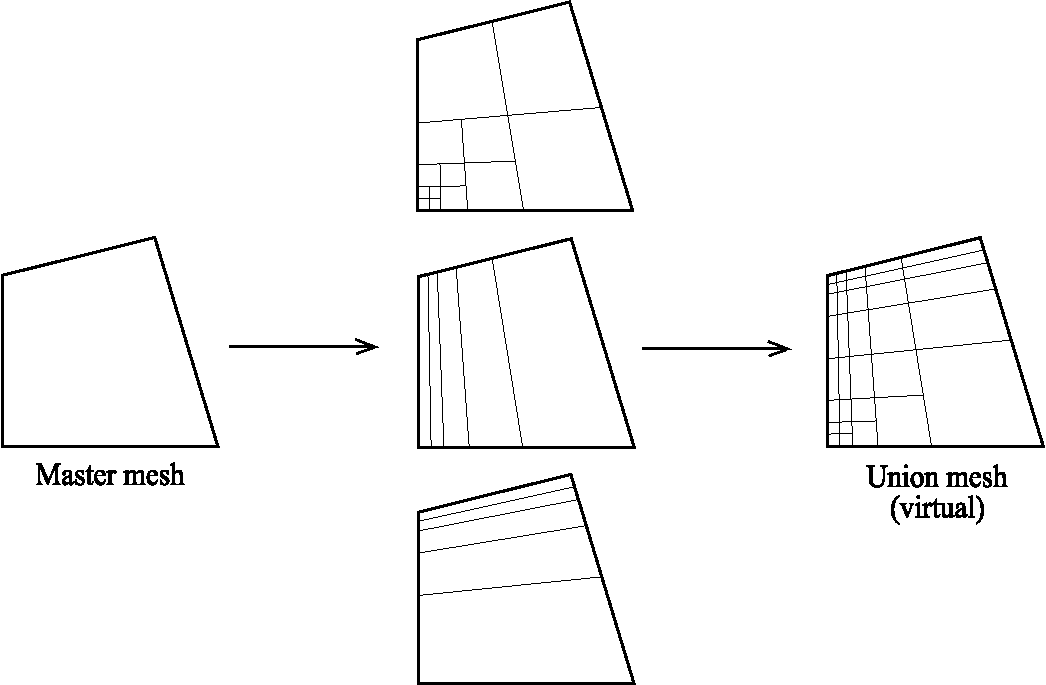
\includegraphics[height=0.7\textheight]{multimesh/multimesh_new.pdf}
  \end{center}
\end{frame}

\begin{frame}
  \frametitle{Monolithic Adaptive Multimesh FEM}
  \begin{center}
    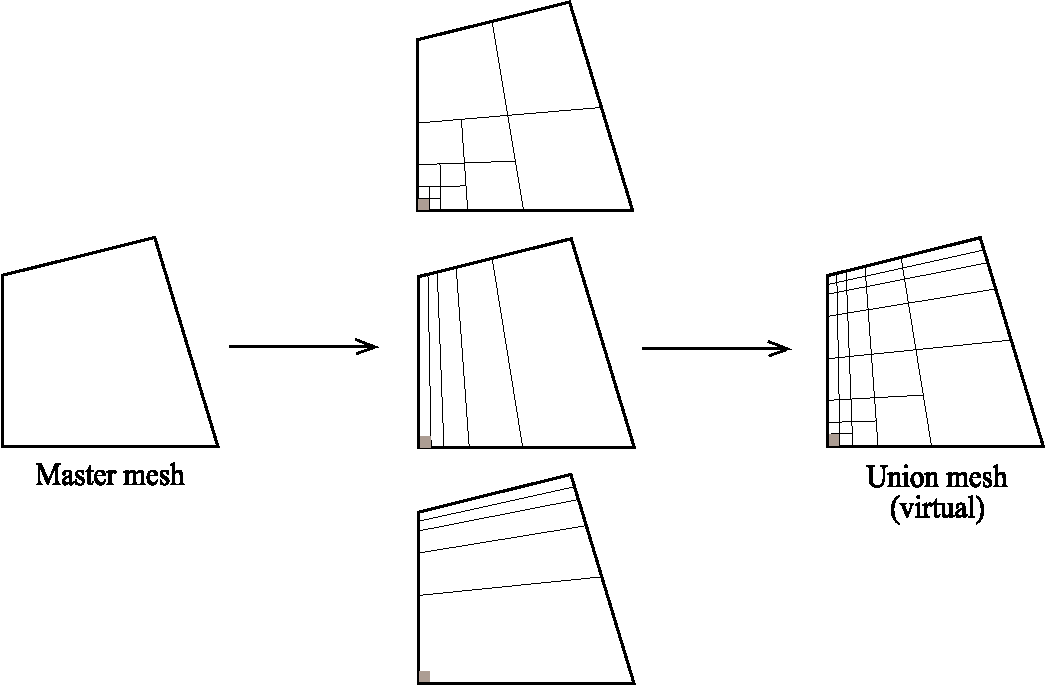
\includegraphics[height=0.7\textheight]{multimesh/mm_1.pdf}
  \end{center}
\end{frame}

\begin{frame}
  \frametitle{Monolithic Adaptive Multimesh FEM}
  \begin{center}
    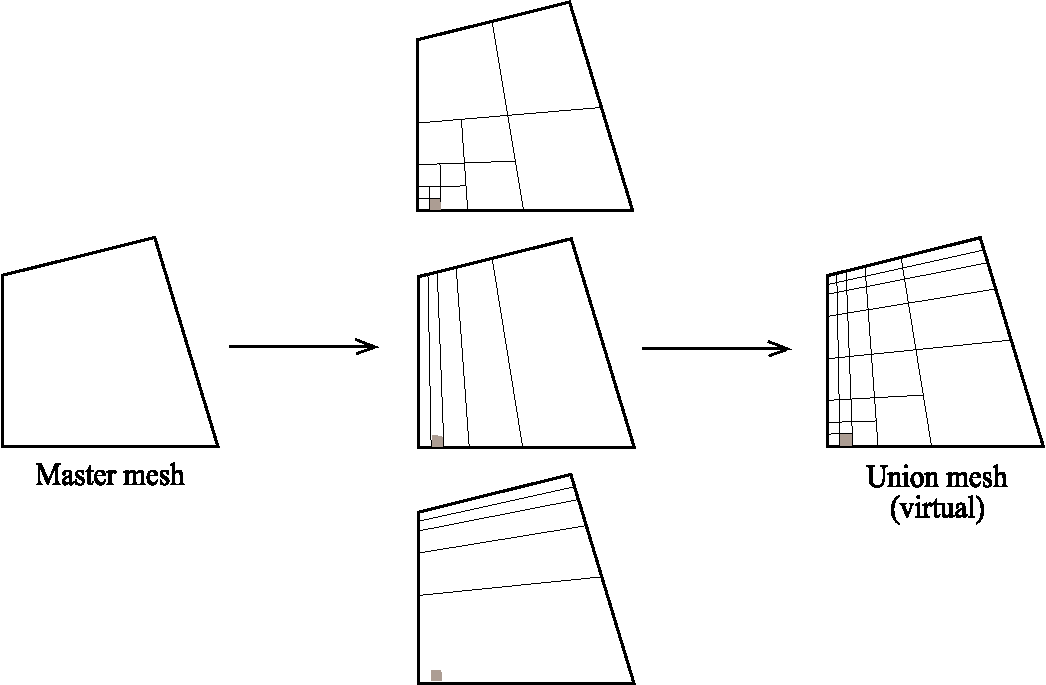
\includegraphics[height=0.7\textheight]{multimesh/mm_2.pdf}
  \end{center}
\end{frame}

\begin{frame}
  \frametitle{Monolithic Adaptive Multimesh FEM}
  \begin{center}
    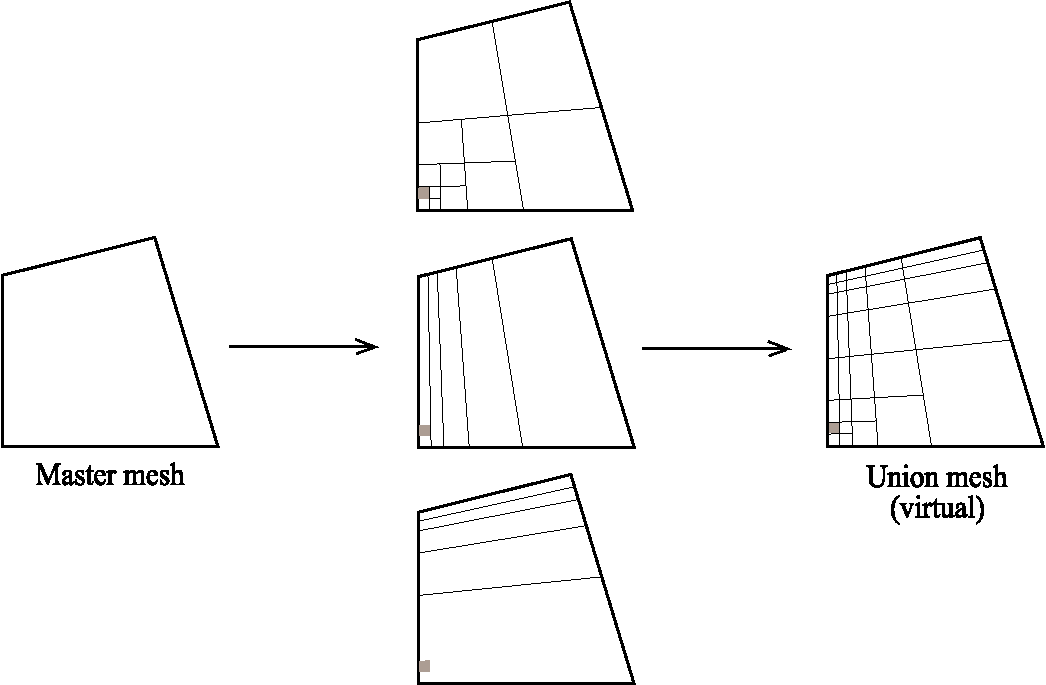
\includegraphics[height=0.7\textheight]{multimesh/mm_3.pdf}
  \end{center}
\end{frame}

\begin{frame}
  \frametitle{Monolithic Adaptive Multimesh FEM}
  \begin{center}
    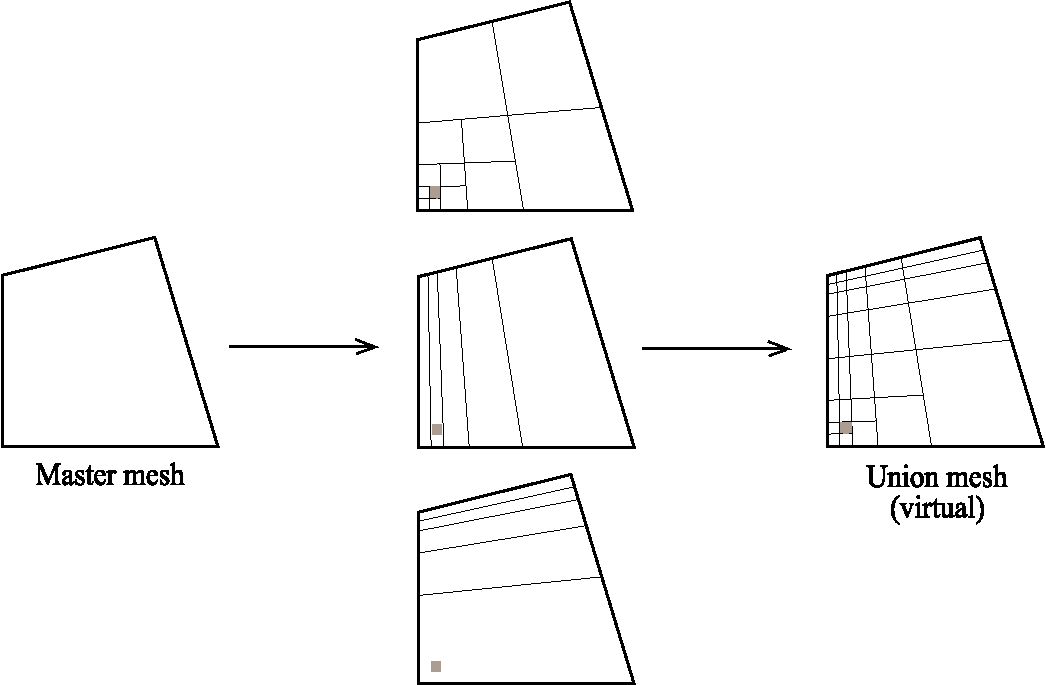
\includegraphics[height=0.7\textheight]{multimesh/mm_4.pdf}
  \end{center}
\end{frame}

\begin{frame}
  \frametitle{Monolithic Adaptive Multimesh FEM}
  \begin{center}
    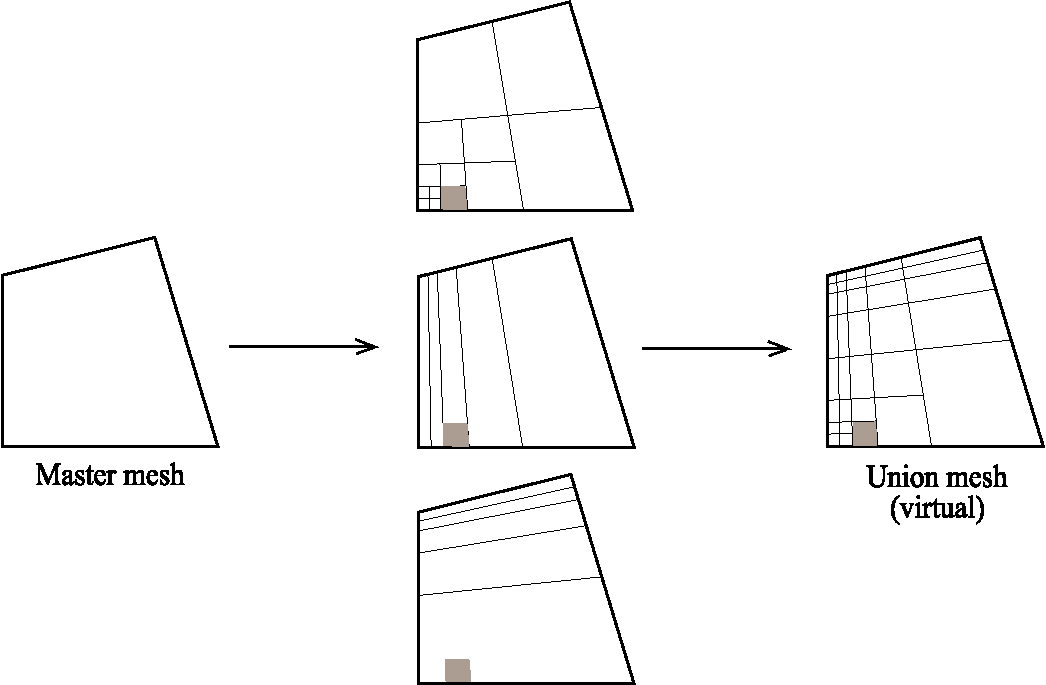
\includegraphics[height=0.7\textheight]{multimesh/mm_5.pdf}
  \end{center}
\end{frame}

\begin{frame}
  \frametitle{Monolithic Adaptive Multimesh FEM}
  \begin{center}
    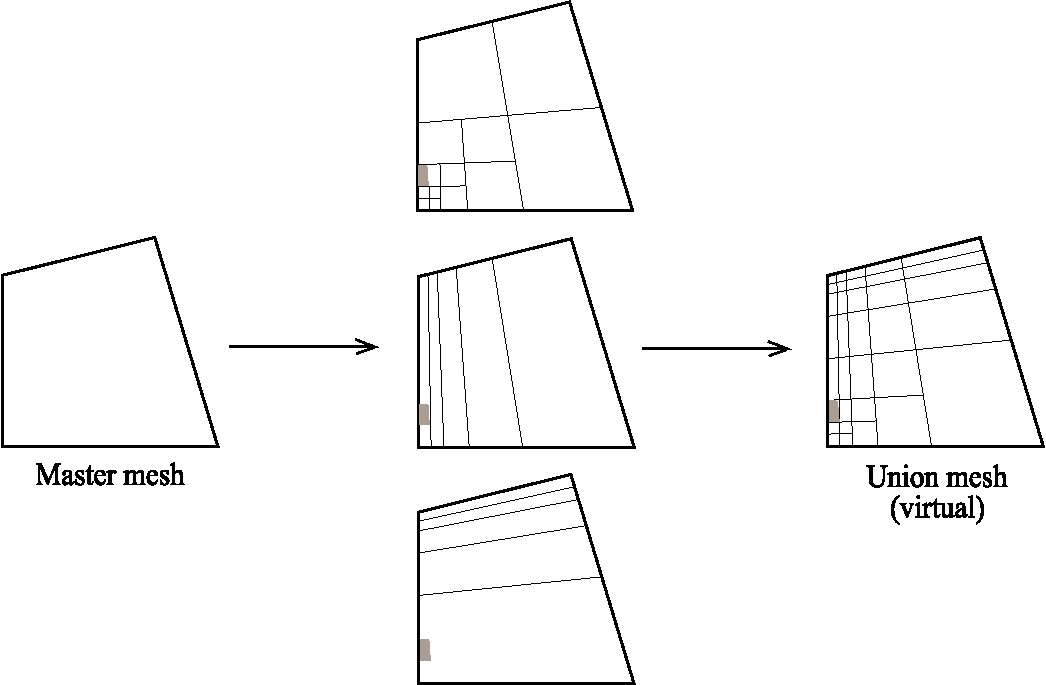
\includegraphics[height=0.7\textheight]{multimesh/mm_6.pdf}
  \end{center}
\end{frame}

\begin{frame}
  \frametitle{Monolithic Adaptive Multimesh FEM}
  \begin{center}
    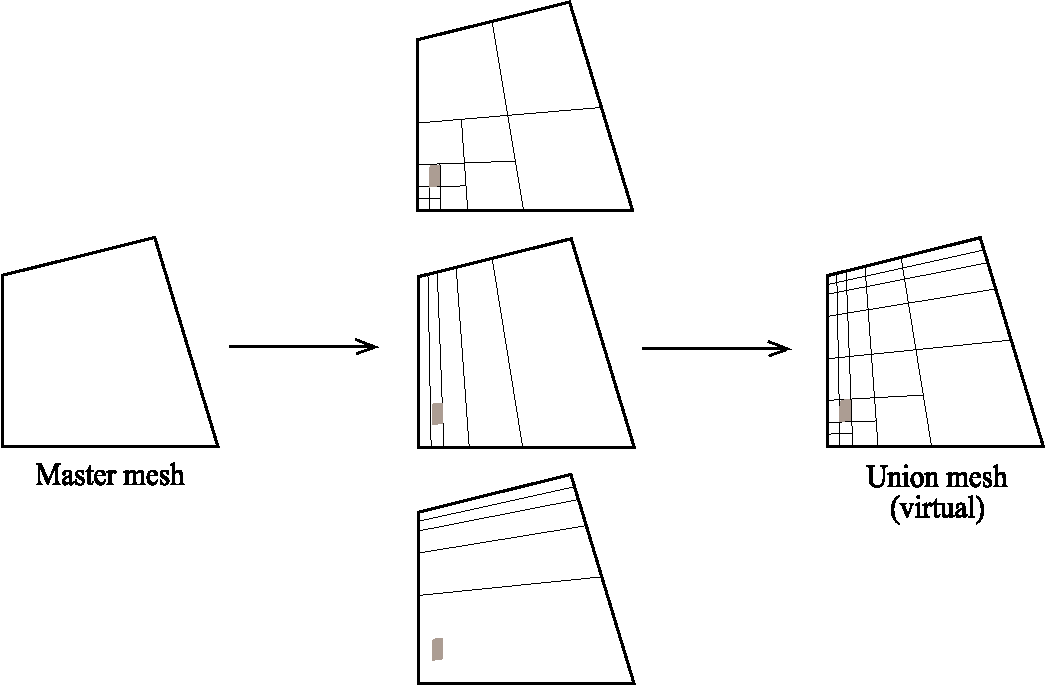
\includegraphics[height=0.7\textheight]{multimesh/mm_7.pdf}
  \end{center}
\end{frame}

\begin{frame}
  \frametitle{Monolithic Adaptive Multimesh FEM}
  \begin{center}
    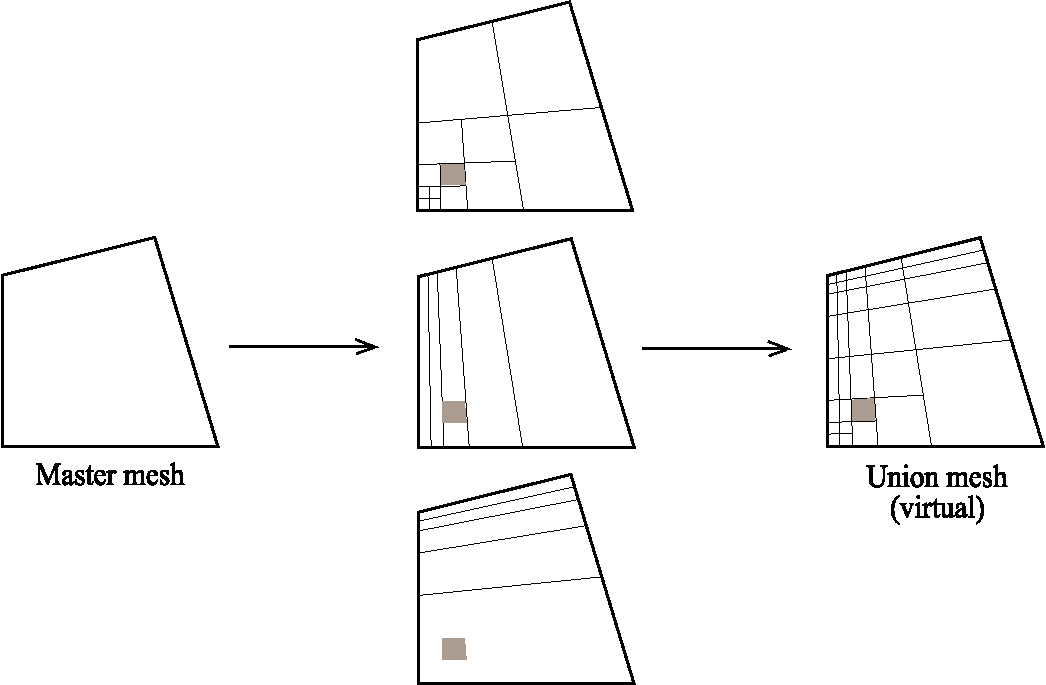
\includegraphics[height=0.7\textheight]{multimesh/mm_8.pdf}
  \end{center}
\end{frame}

\begin{frame}
  \frametitle{Monolithic Adaptive Multimesh FEM}
  \begin{center}
    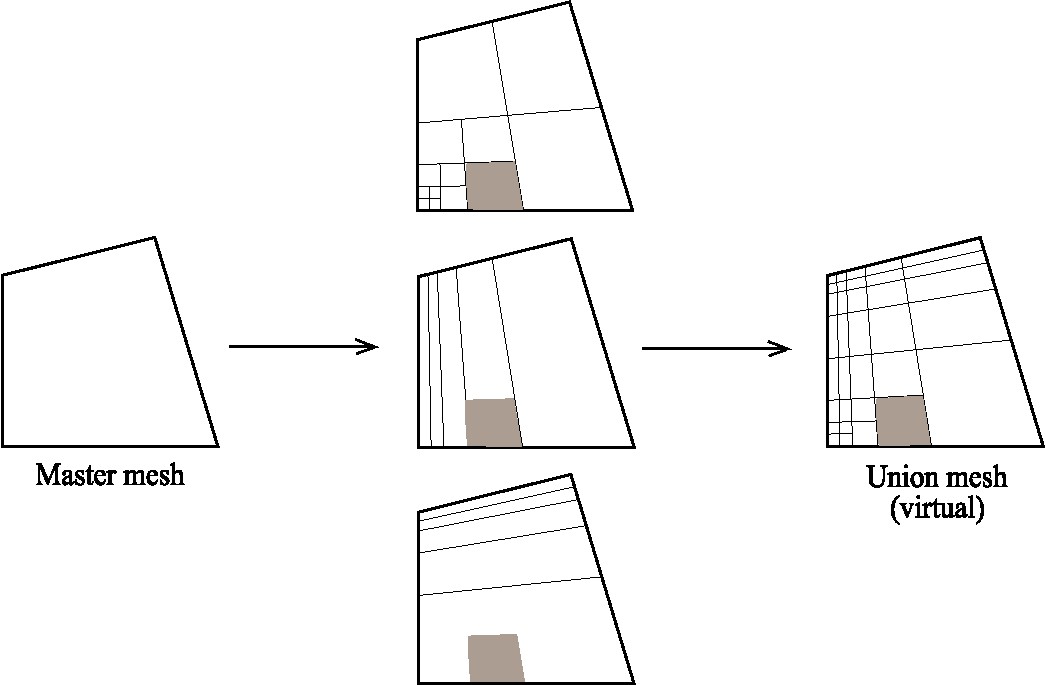
\includegraphics[height=0.7\textheight]{multimesh/mm_9.pdf}
  \end{center}
\end{frame}

\begin{frame}
  \frametitle{Monolithic Adaptive Multimesh FEM}
  \begin{center}
    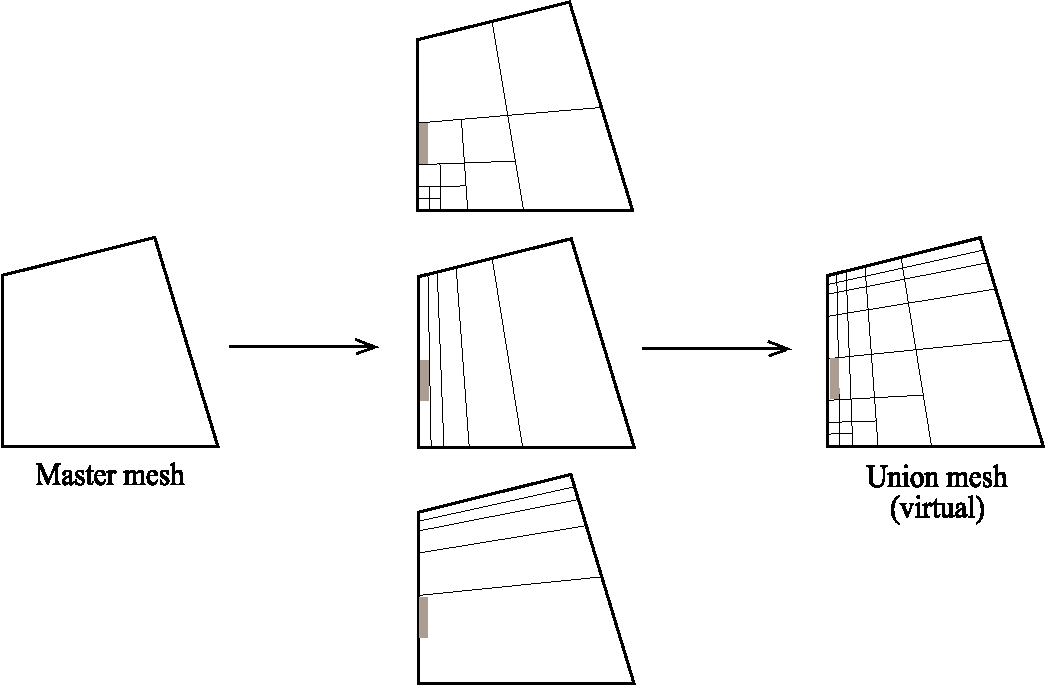
\includegraphics[height=0.7\textheight]{multimesh/mm_10.pdf}
  \end{center}
\end{frame}

\begin{frame}
  \frametitle{Monolithic Adaptive Multimesh FEM}
  \begin{center}
    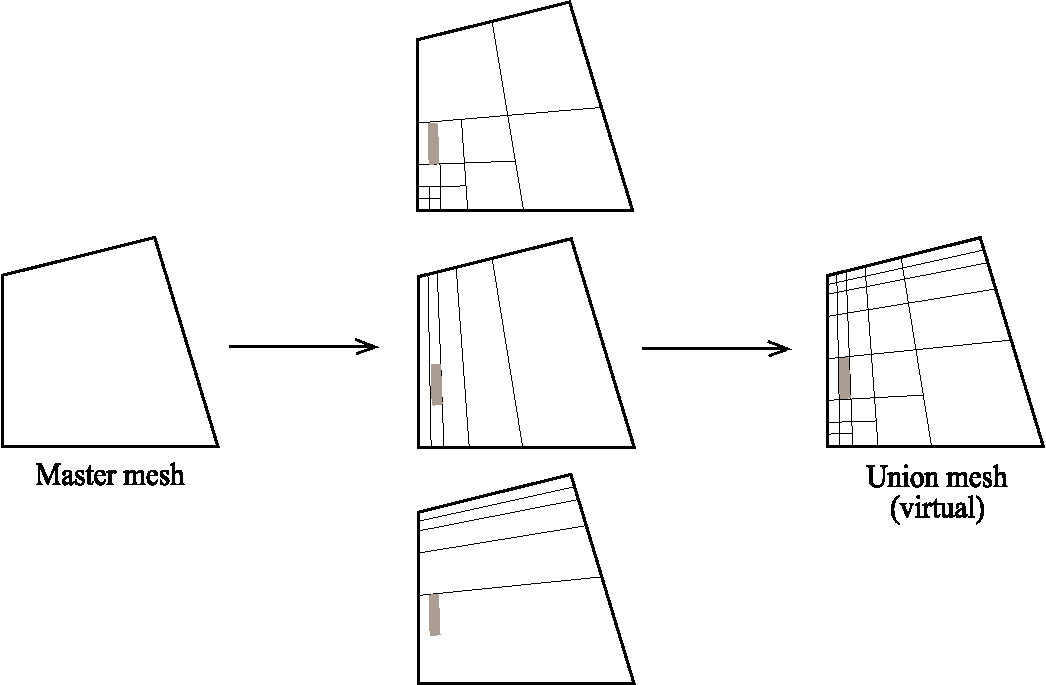
\includegraphics[height=0.7\textheight]{multimesh/mm_11.pdf}
  \end{center}
\end{frame}

\begin{frame}
  \frametitle{Monolithic Adaptive Multimesh FEM}
  \begin{center}
    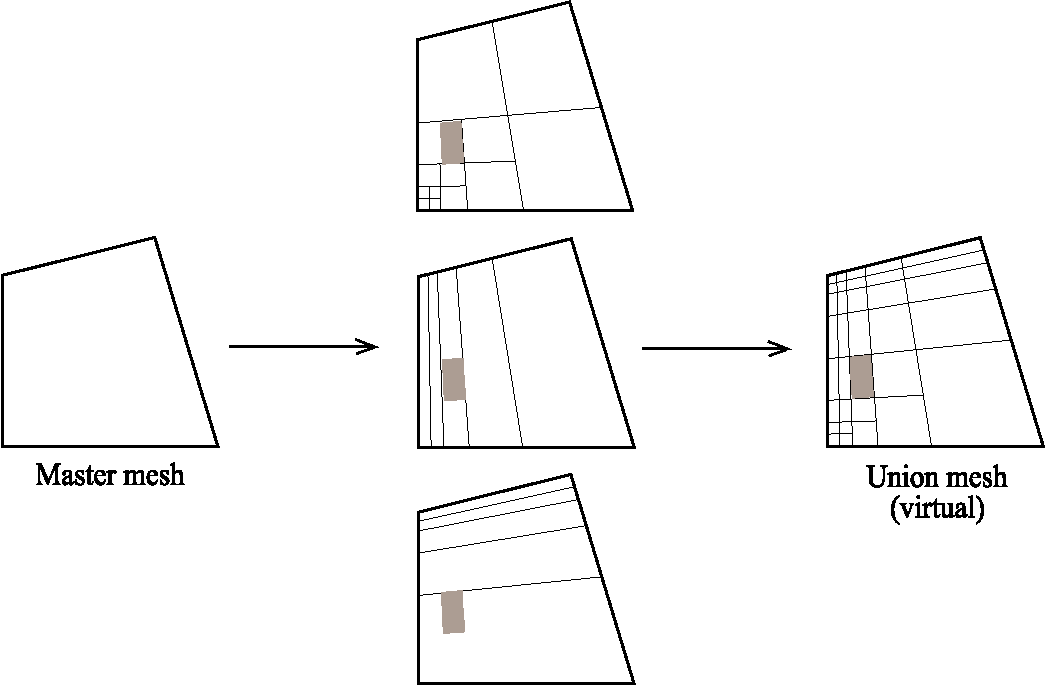
\includegraphics[height=0.7\textheight]{multimesh/mm_12.pdf}
  \end{center}
\end{frame}

\begin{frame}
  \frametitle{Monolithic Adaptive Multimesh FEM}
  \begin{center}
    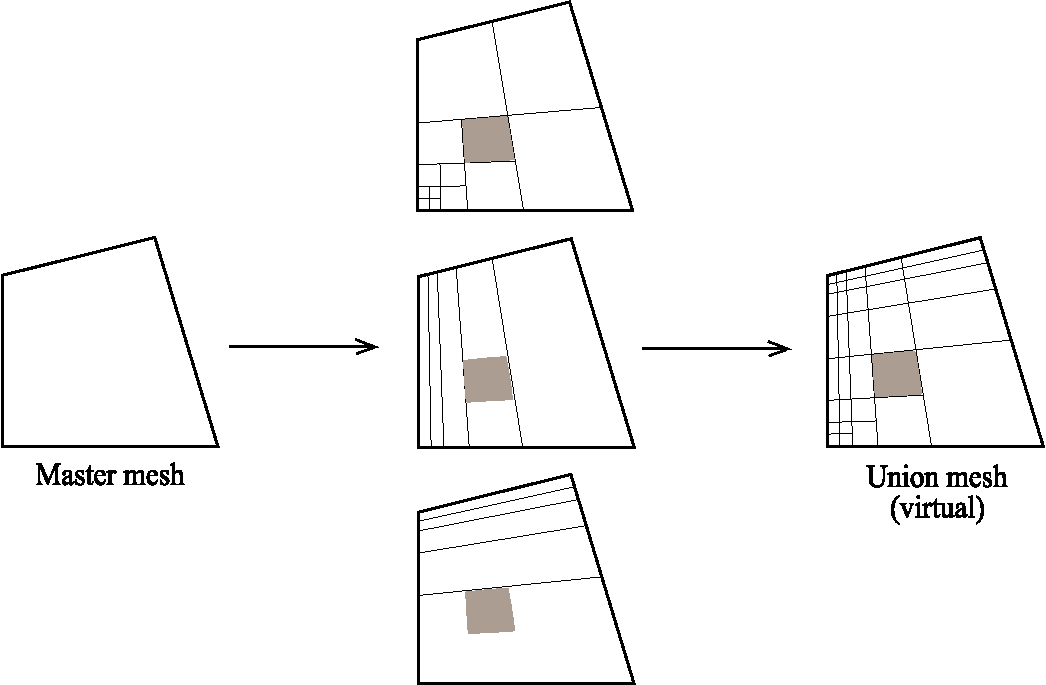
\includegraphics[height=0.7\textheight]{multimesh/mm_13.pdf}
  \end{center}
\end{frame}

\begin{frame}
  \frametitle{Monolithic Adaptive Multimesh FEM}
  \begin{center}
    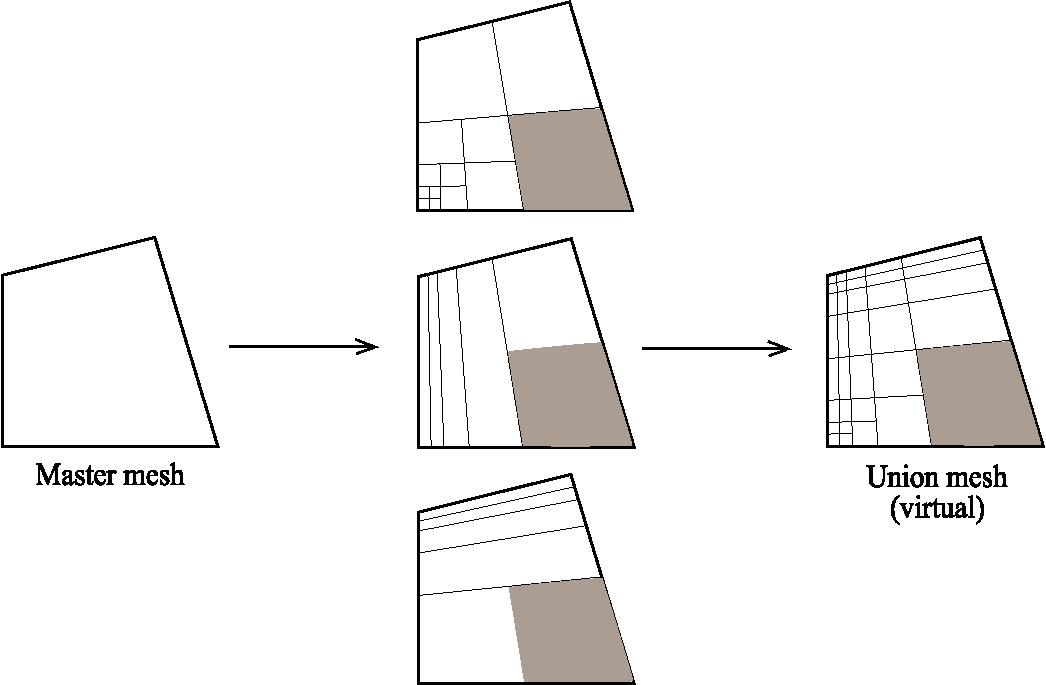
\includegraphics[height=0.7\textheight]{multimesh/mm_14.pdf}
  \end{center}
\end{frame}

\begin{frame}
  \frametitle{Monolithic Adaptive Multimesh FEM}
  \begin{center}
    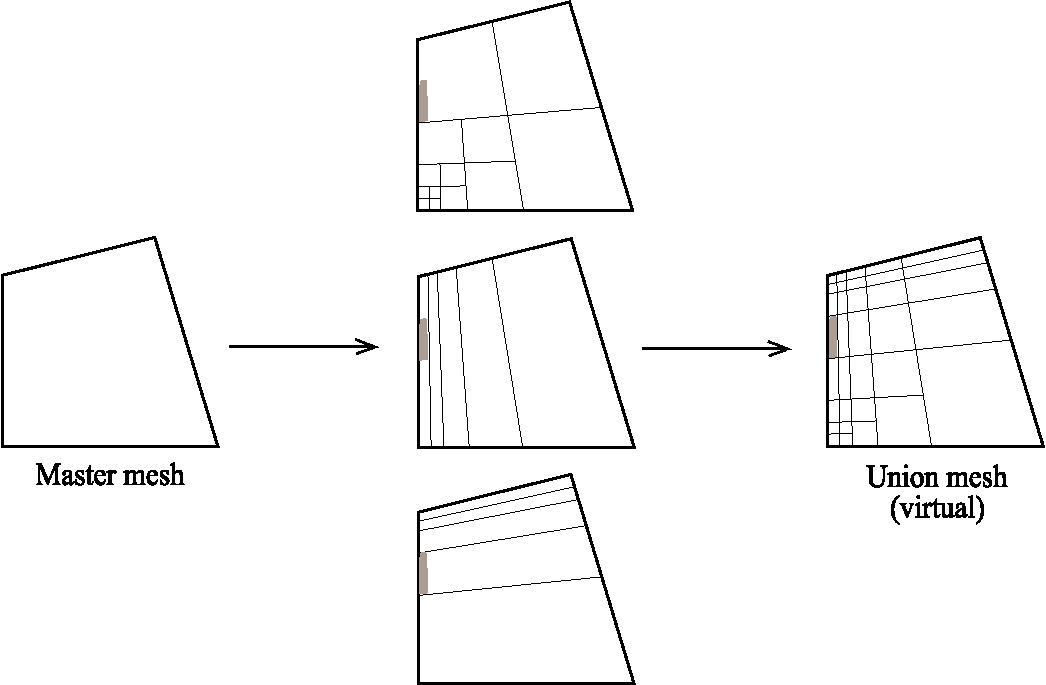
\includegraphics[height=0.7\textheight]{multimesh/mm_15.pdf}
  \end{center}
\end{frame}

\begin{frame}
  \frametitle{Monolithic Adaptive Multimesh FEM}
  \begin{center}
    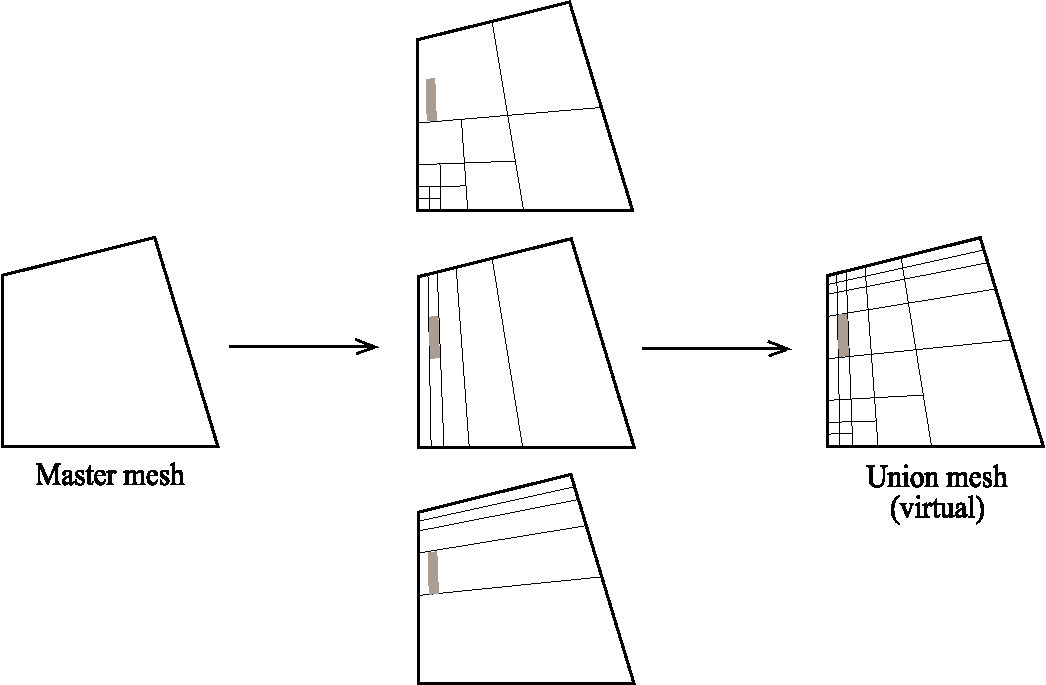
\includegraphics[height=0.7\textheight]{multimesh/mm_16.pdf}
  \end{center}
\end{frame}

\begin{frame}
  \frametitle{Monolithic Adaptive Multimesh FEM}
  \begin{center}
    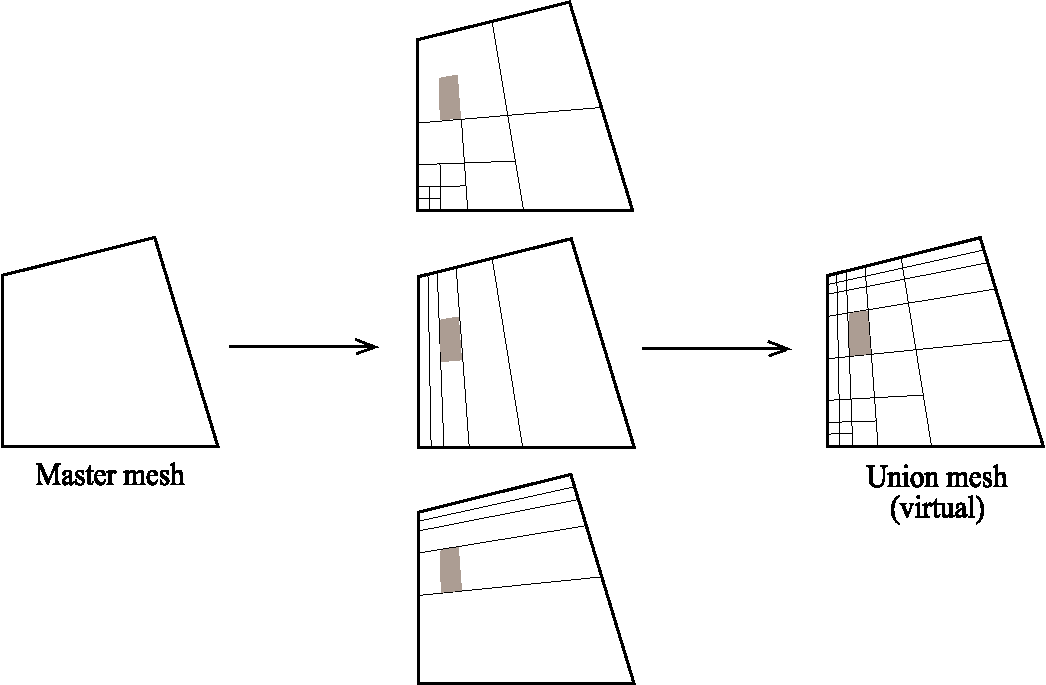
\includegraphics[height=0.7\textheight]{multimesh/mm_17.pdf}
  \end{center}
\end{frame}

\begin{frame}
  \frametitle{Monolithic Adaptive Multimesh FEM}
  \begin{center}
    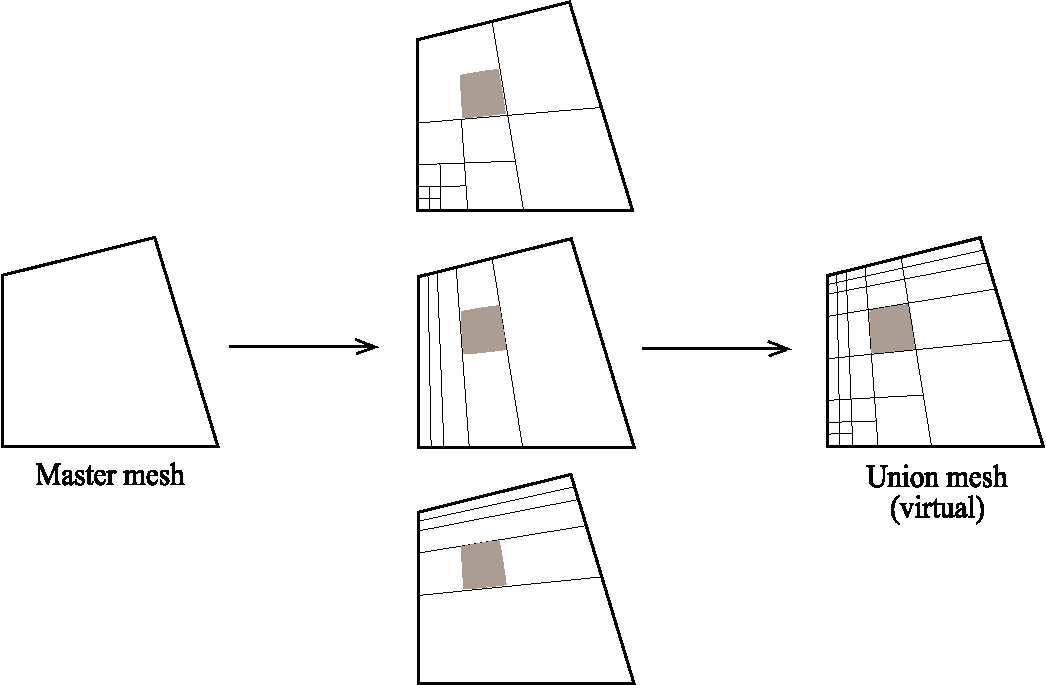
\includegraphics[height=0.7\textheight]{multimesh/mm_18.pdf}
  \end{center}
\end{frame}

\begin{frame}
  \frametitle{Monolithic Adaptive Multimesh FEM}
  \begin{center}
    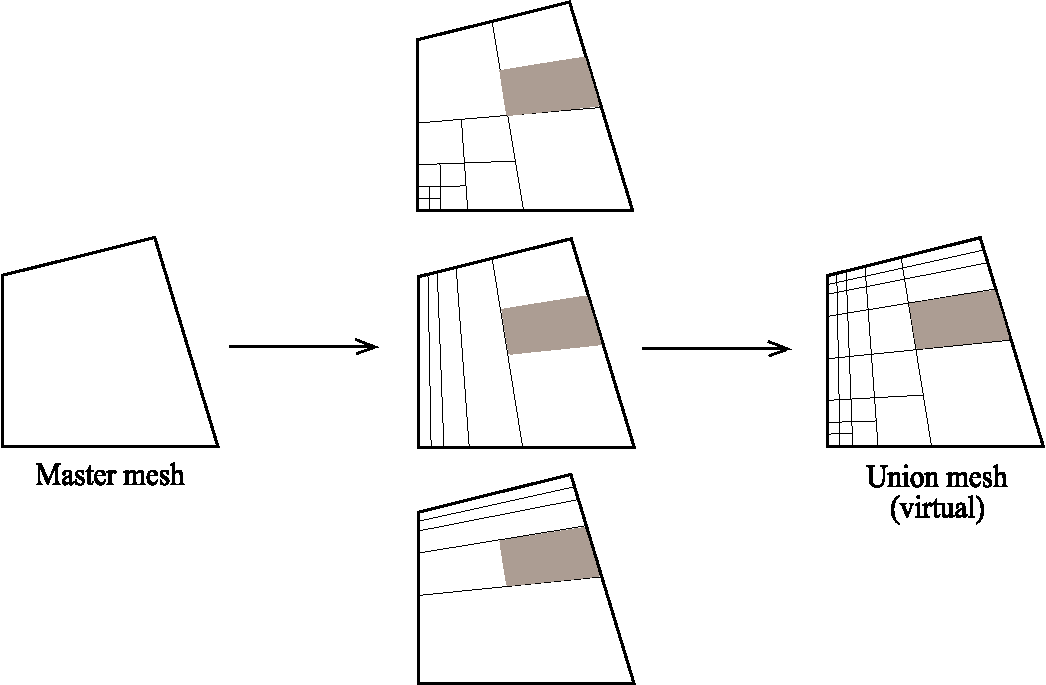
\includegraphics[height=0.7\textheight]{multimesh/mm_19.pdf}
  \end{center}
\end{frame}

\begin{frame}
  \frametitle{Monolithic Adaptive Multimesh FEM}
  \begin{center}
    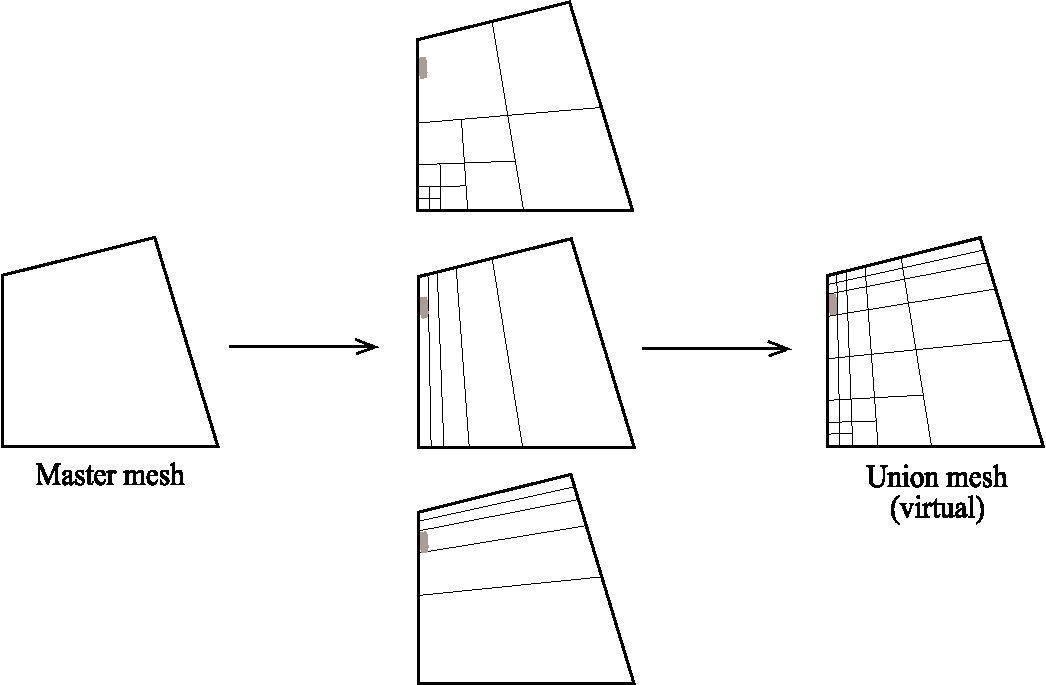
\includegraphics[height=0.7\textheight]{multimesh/mm_20.pdf}
  \end{center}
\end{frame}

\begin{frame}
  \frametitle{Monolithic Adaptive Multimesh FEM}
  \begin{center}
    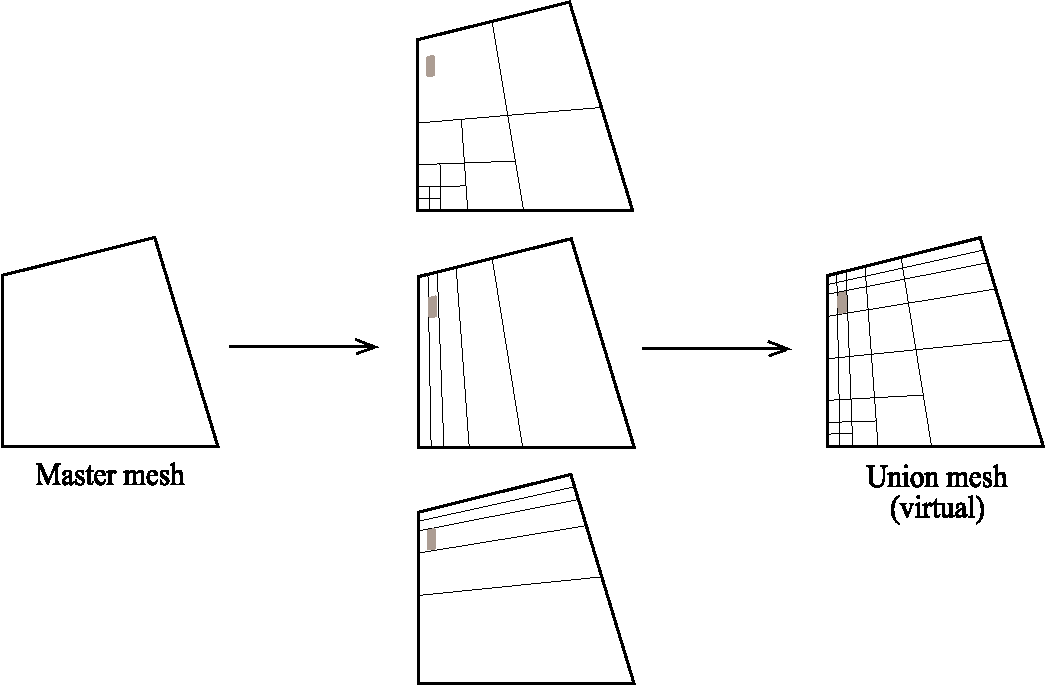
\includegraphics[height=0.7\textheight]{multimesh/mm_21.pdf}
  \end{center}
\end{frame}

\begin{frame}
  \frametitle{Monolithic Adaptive Multimesh FEM}
  \begin{center}
    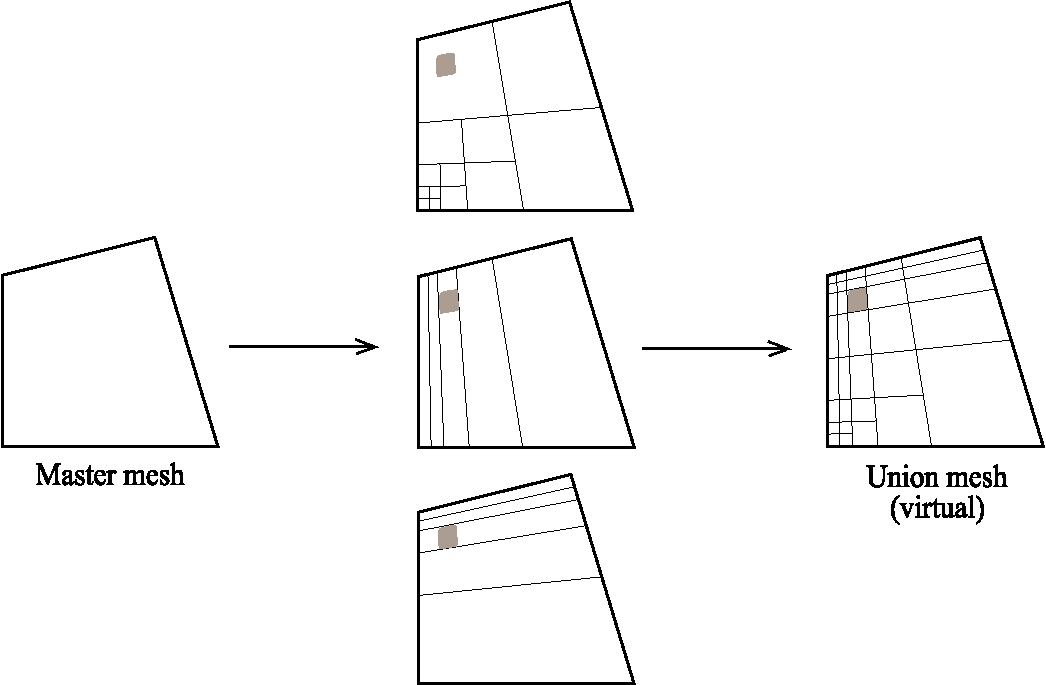
\includegraphics[height=0.7\textheight]{multimesh/mm_22.pdf}
  \end{center}
\end{frame}

\begin{frame}
  \frametitle{Monolithic Adaptive Multimesh FEM}
  \begin{center}
    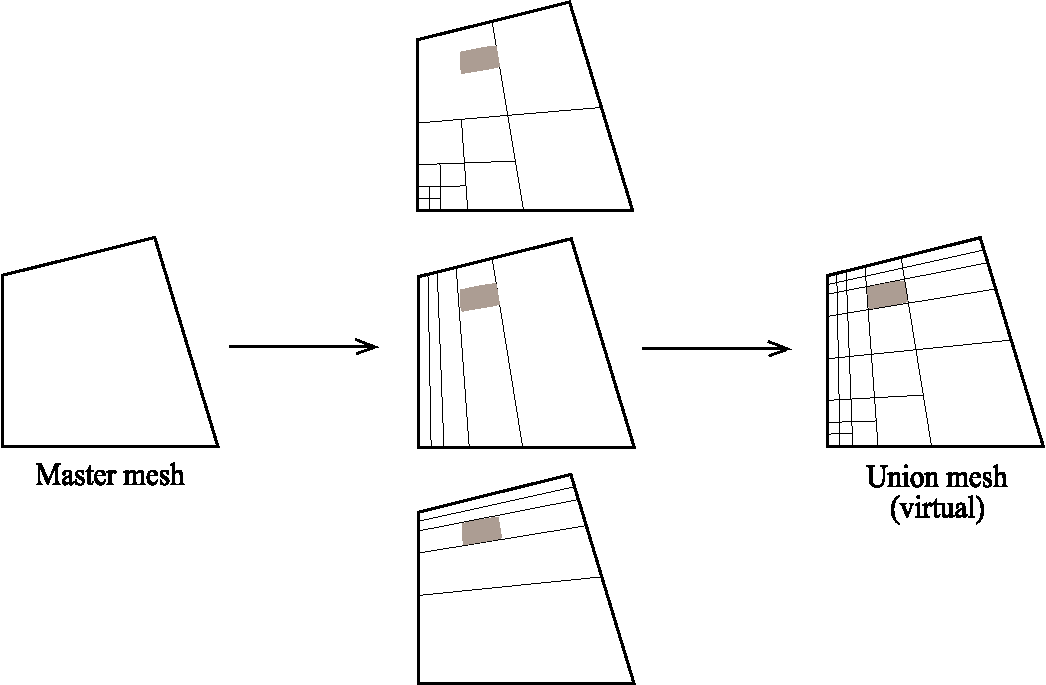
\includegraphics[height=0.7\textheight]{multimesh/mm_23.pdf}
  \end{center}
\end{frame}

\begin{frame}
  \frametitle{Monolithic Adaptive Multimesh FEM}
  \begin{center}
    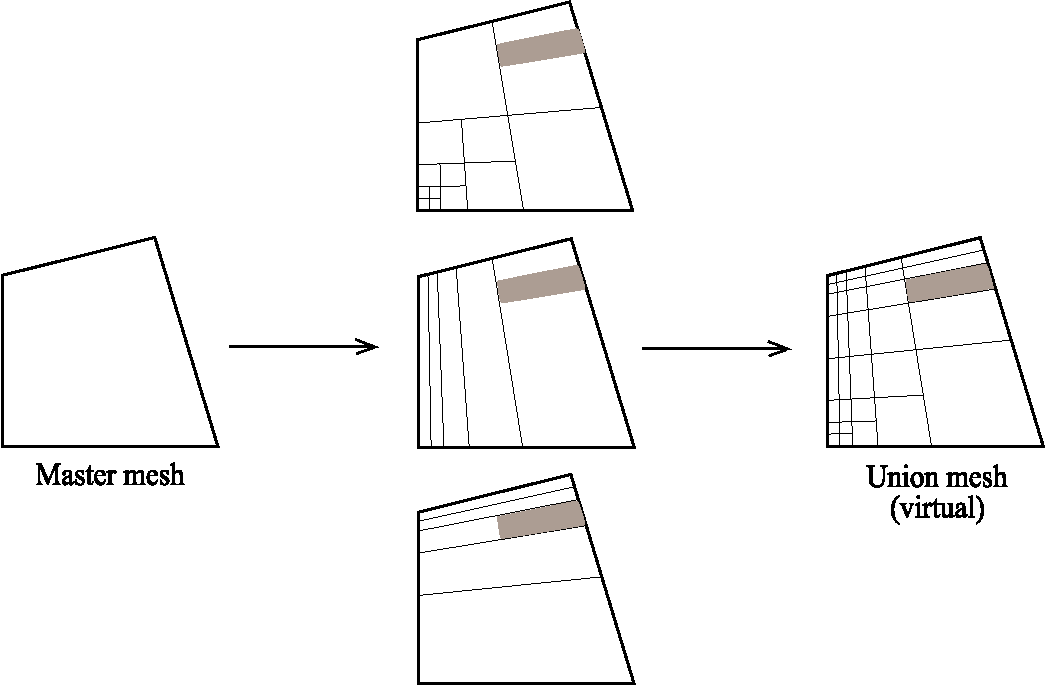
\includegraphics[height=0.7\textheight]{multimesh/mm_24.pdf}
  \end{center}
\end{frame}

\begin{frame}
  \frametitle{Monolithic Adaptive Multimesh FEM}
  \begin{center}
    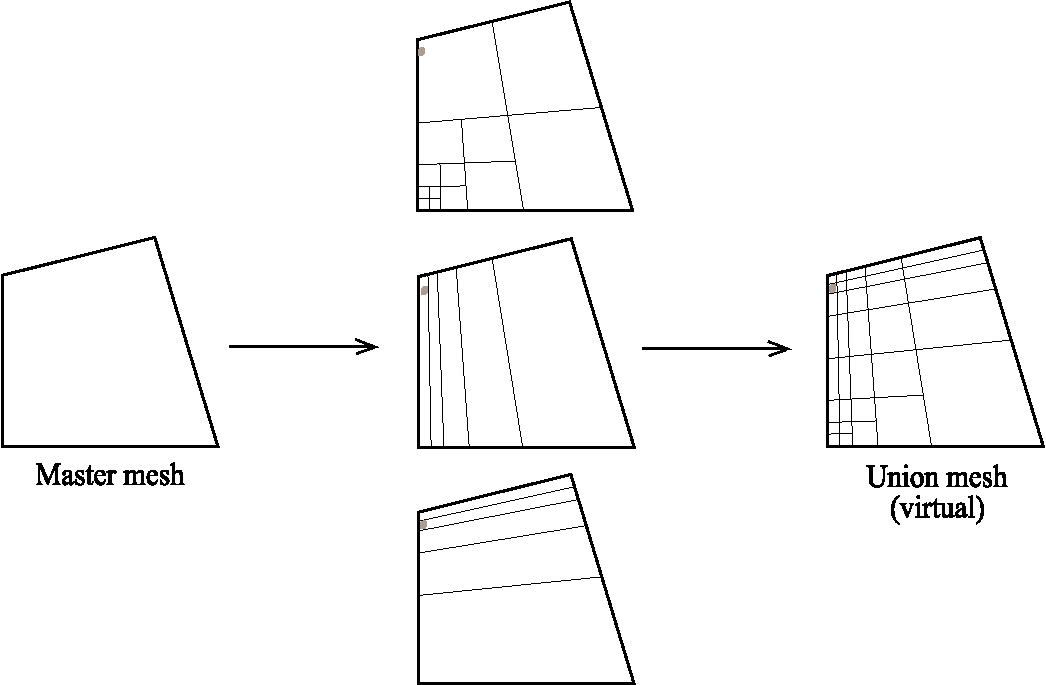
\includegraphics[height=0.7\textheight]{multimesh/mm_25.pdf}
  \end{center}
\end{frame}

\begin{frame}
  \frametitle{Monolithic Adaptive Multimesh FEM}
  \begin{center}
    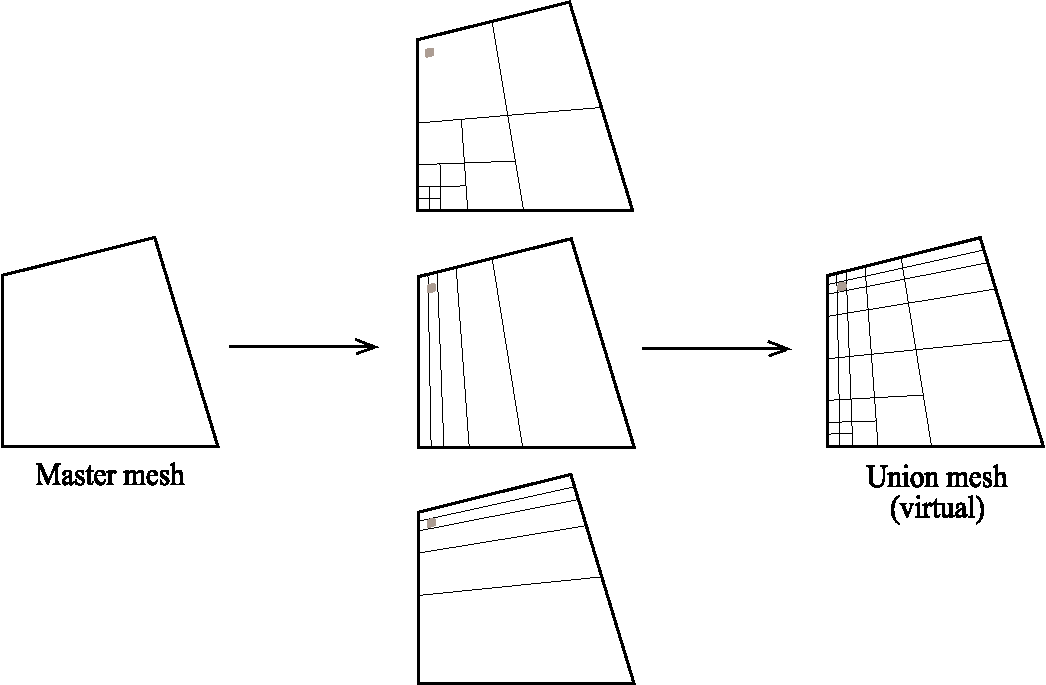
\includegraphics[height=0.7\textheight]{multimesh/mm_26.pdf}
  \end{center}
\end{frame}

\begin{frame}
  \frametitle{Monolithic Adaptive Multimesh FEM}
  \begin{center}
    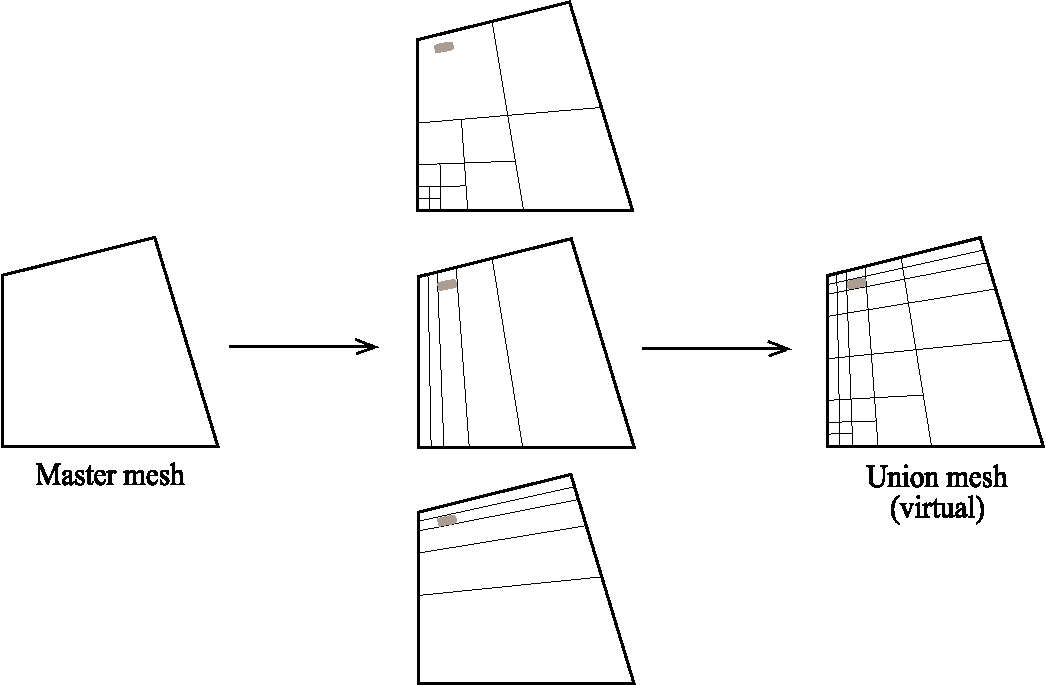
\includegraphics[height=0.7\textheight]{multimesh/mm_27.pdf}
  \end{center}
\end{frame}

\begin{frame}
  \frametitle{Monolithic Adaptive Multimesh FEM}
  \begin{center}
    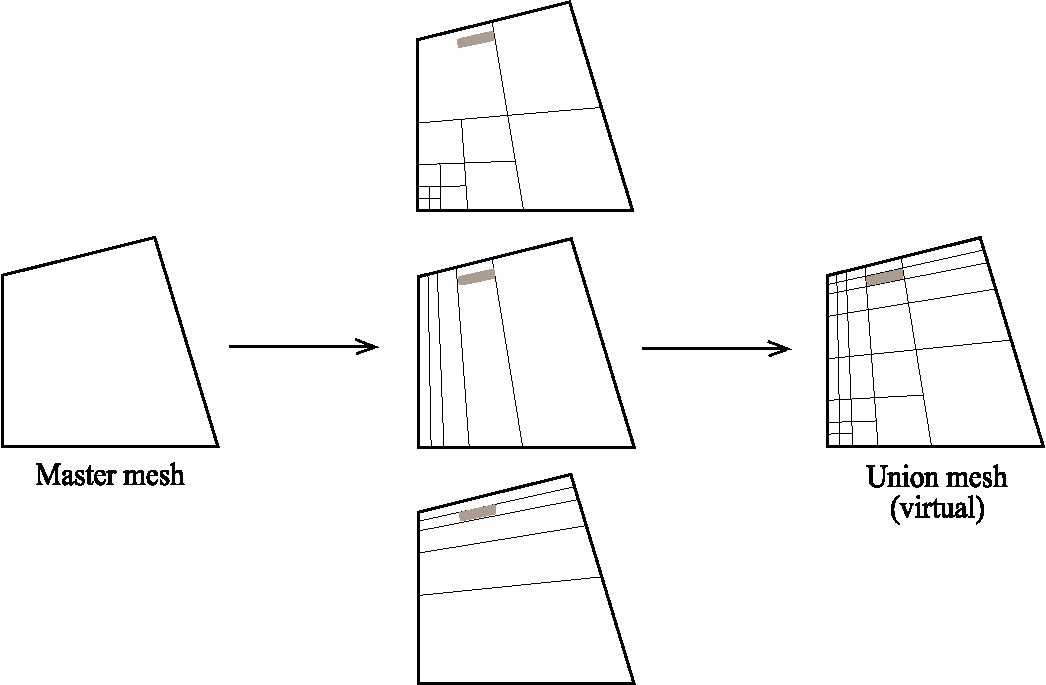
\includegraphics[height=0.7\textheight]{multimesh/mm_28.pdf}
  \end{center}
\end{frame}

\begin{frame}
  \frametitle{Monolithic Adaptive Multimesh FEM}
  \begin{center}
    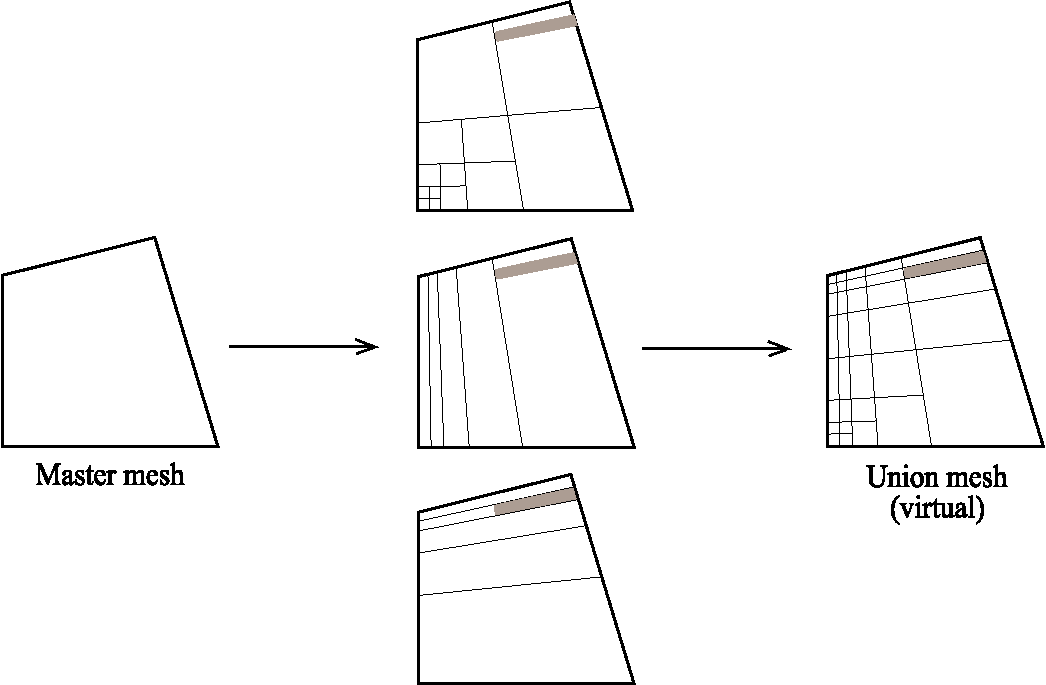
\includegraphics[height=0.7\textheight]{multimesh/mm_29.pdf}
  \end{center}
\end{frame}

\begin{frame}
  \frametitle{Monolithic Adaptive Multimesh FEM}
  \begin{center}
    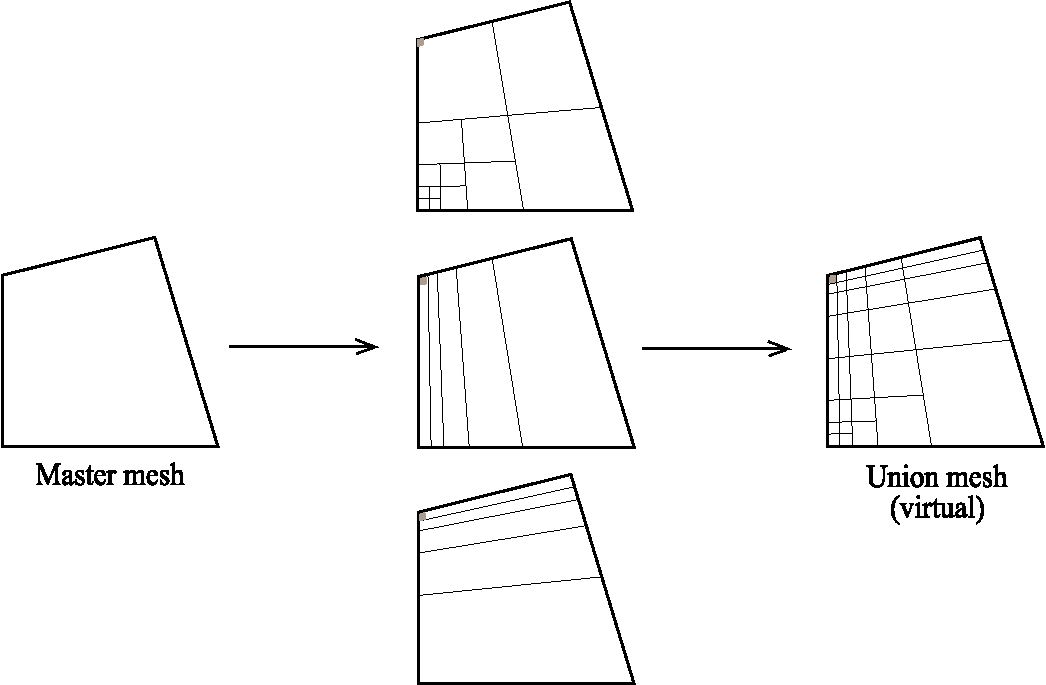
\includegraphics[height=0.7\textheight]{multimesh/mm_30.pdf}
  \end{center}
\end{frame}

\begin{frame}
  \frametitle{Monolithic Adaptive Multimesh FEM}
  \begin{center}
    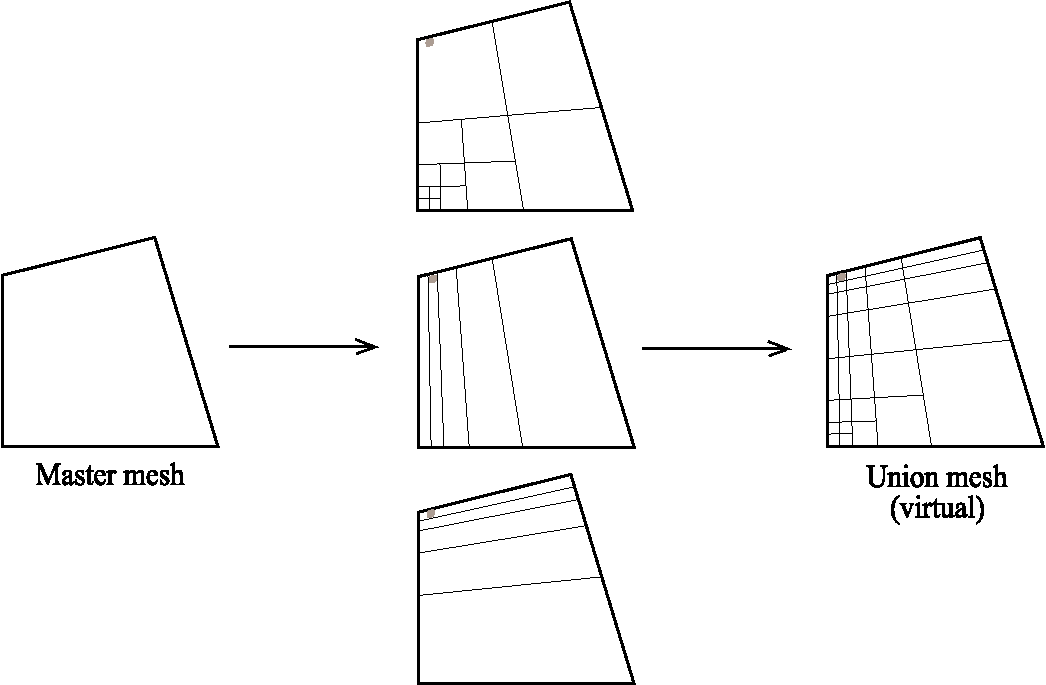
\includegraphics[height=0.7\textheight]{multimesh/mm_31.pdf}
  \end{center}
\end{frame}

\begin{frame}
  \frametitle{Monolithic Adaptive Multimesh FEM}
  \begin{center}
    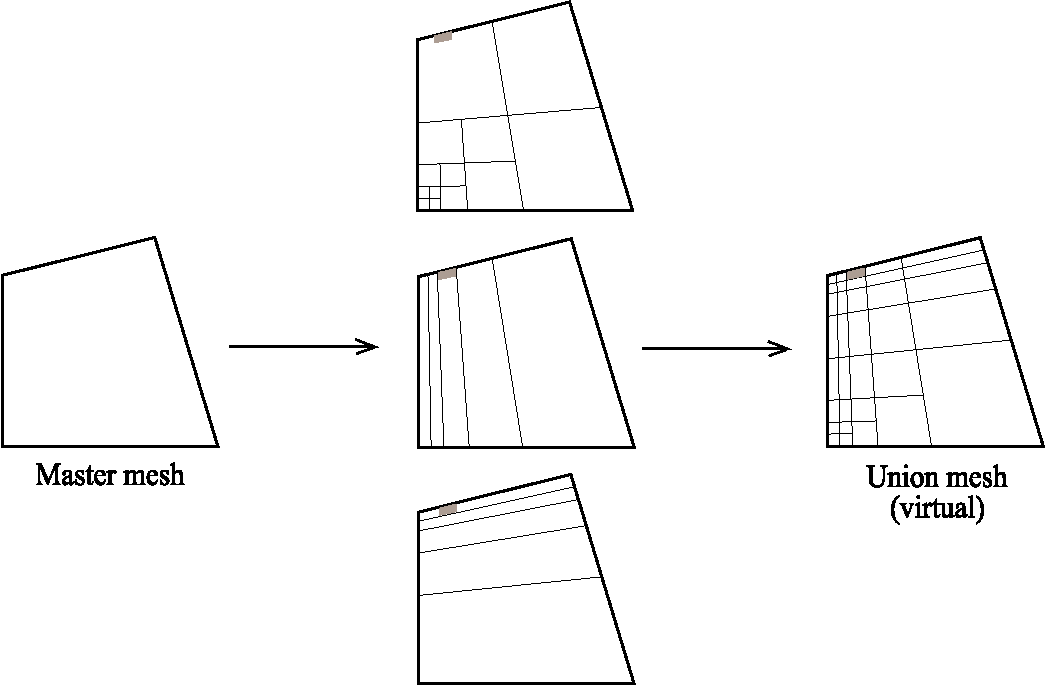
\includegraphics[height=0.7\textheight]{multimesh/mm_32.pdf}
  \end{center}
\end{frame}

\begin{frame}
  \frametitle{Monolithic Adaptive Multimesh FEM}
  \begin{center}
    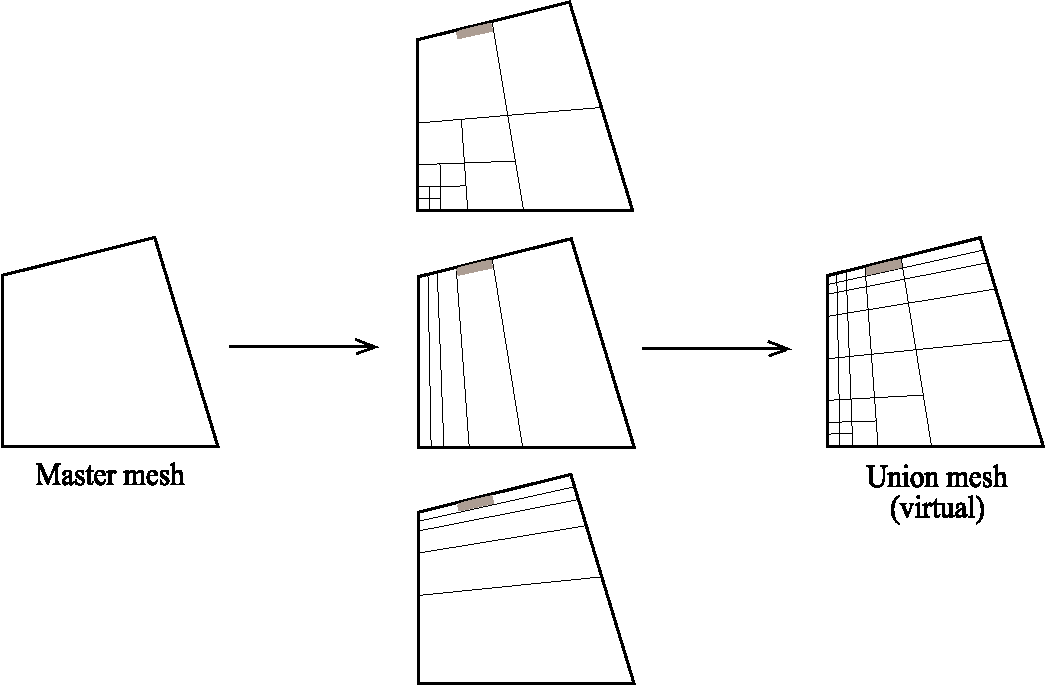
\includegraphics[height=0.7\textheight]{multimesh/mm_33.pdf}
  \end{center}
\end{frame}

\begin{frame}
  \frametitle{Monolithic Adaptive Multimesh FEM}
  \begin{center}
    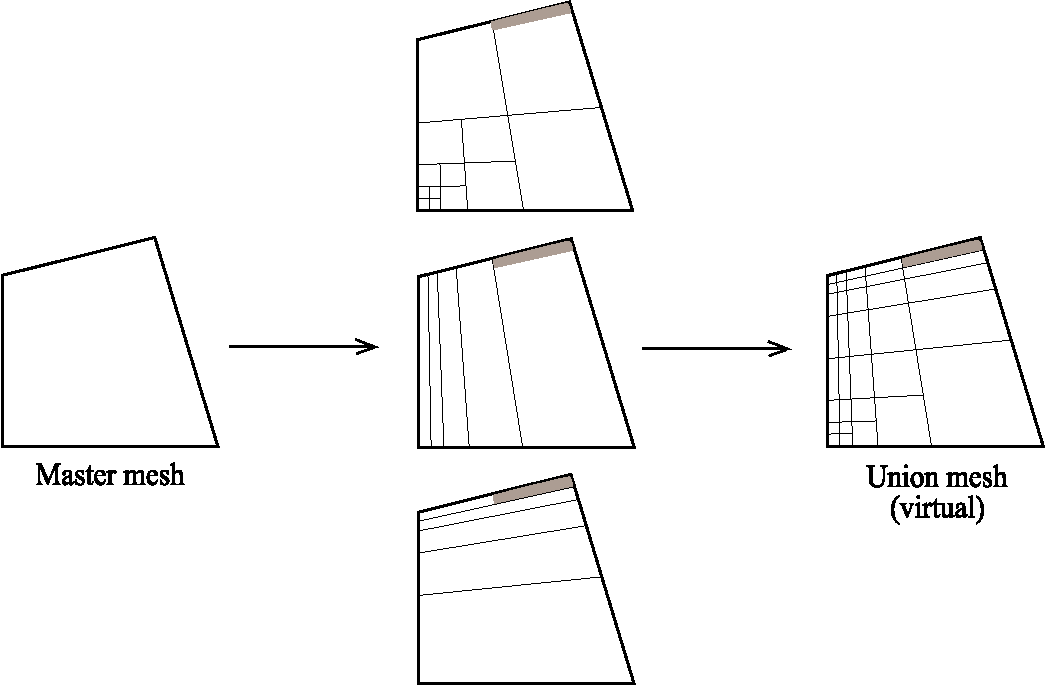
\includegraphics[height=0.7\textheight]{multimesh/mm_34.pdf}
  \end{center}
\end{frame}


%Arbitrary-level hanging nodes
\begin{frame}
  \frametitle{Hanging nodes}
\end{frame}

\begin{frame}
  \frametitle{Hanging nodes}
\vspace{-2.0cm}
  \begin{itemize}
    \item Regular mesh\\[2mm]    
    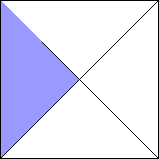
\includegraphics[height=0.3\textheight]{regular_a}
  \end{itemize}
\end{frame}

\begin{frame}
\vspace{-2.0cm}
  \frametitle{Hanging nodes}
  \begin{itemize}
    \item Regular mesh\\[2mm]    
    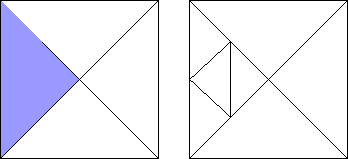
\includegraphics[height=0.3\textheight]{regular_b}
  \end{itemize}
\end{frame}

\begin{frame}
\vspace{-2.0cm}
  \frametitle{Hanging nodes}
  \begin{itemize}
    \item Regular mesh\\[2mm]    
    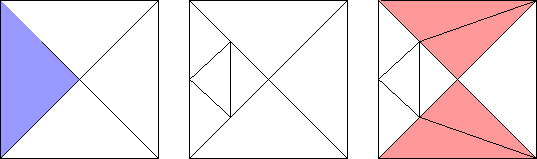
\includegraphics[height=0.3\textheight]{regular_c}
  \end{itemize}
\end{frame}

\begin{frame}
  \frametitle{Hanging nodes}
  \begin{itemize}
    \item Regular mesh\\[2mm]    
    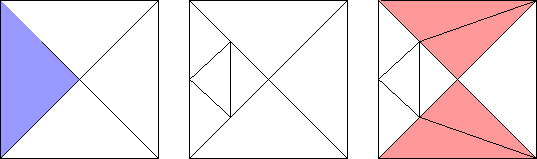
\includegraphics[height=0.3\textheight]{regular_c}
    \item One-level hanging nodes (1-irregular mesh)\\[2mm]   
    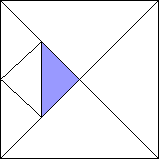
\includegraphics[height=0.3\textheight]{one_irr_a}
  \end{itemize}
\end{frame}

\begin{frame}
  \frametitle{Hanging nodes}
  \begin{itemize}
    \item Regular mesh\\[2mm]    
    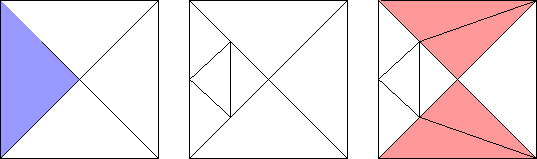
\includegraphics[height=0.3\textheight]{regular_c}
    \item One-level hanging nodes (1-irregular mesh)\\[2mm]   
    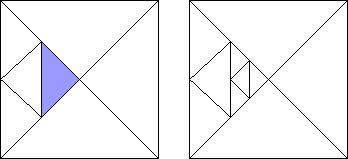
\includegraphics[height=0.3\textheight]{one_irr_b}
  \end{itemize}
\end{frame}

\begin{frame}
  \frametitle{Hanging nodes}
  \begin{itemize}
    \item Regular mesh\\[2mm]    
    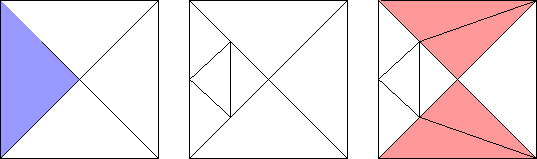
\includegraphics[height=0.3\textheight]{regular_c}
    \item One-level hanging nodes (1-irregular mesh)\\[2mm]
    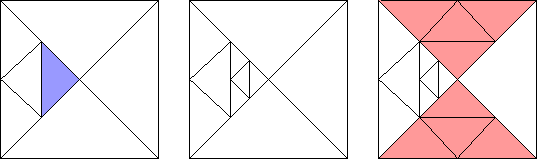
\includegraphics[height=0.3\textheight]{one_irr_c}
  \end{itemize}
\end{frame} 

\begin{frame}
\frametitle{Hanging nodes}
\begin{itemize}
\item Forced refinements
\begin{itemize}
\item introduce unnecessary DOF
\item spoil element shapes
\item have recursive nature
\item cause incompatible refinements in the multi-mesh $hp$-FEM
\end{itemize}
\item Arbitrary-level hanging nodes:
\end{itemize}
\begin{figure}[!ht]
\vspace{-1mm}
\begin{center}
    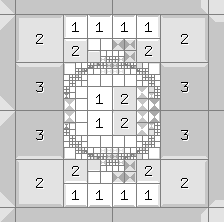
\includegraphics[width=0.25\textwidth]{mesh_irreg2.png}
\end{center}
\noindent
\vspace{-4mm}
\end{figure}
\noindent
{\em P.S., J. Cerveny, I. Dolezel: Arbitrary-Level Hanging Nodes and Automatic
Adaptivity in the hp-FEM, Math. Comput. Simul. 77 (2008), 117 - 132.}
\end{frame}


%Different spaces
\begin{frame}
\frametitle{Component specific function spaces}
\end{frame}

\begin{frame}
\frametitle{Component specific function spaces}
Mathematically, solutions of different equations lie in different function spaces, e.g.
\begin{itemize}
\item Temperature, displacement, etc. - $H^1\ \left(H^2, ..\right)$.
\item Electromagnetics - $H_{curl}$ (discontinuous vector fields with continuous tangential components along all mesh edges $\sim$ gradients of $H^1$ functions).
\item Magnetism - $H_{div}$ (discontinuous vector fields with continuous normal components along all mesh edges $\sim$ divergences of $H^1$ functions).
\item Pressure (in Navier-Stokes equations) - $L^2$.
\end{itemize}
\end{frame}

%Compressible flow -> need for DG
\begin{frame}
\begin{center}
What about compressible flow? $H^1$ too small, $L^2$ too big.\\
\vspace{1cm}
Discontinuous Galerkin method\\\ \\
\begin{itemize}
\item discontinuous piecewise polynomial approximation
\item local character
\item well suited for conservation laws
\item the non-uniqueness of the solution on mesh edges is handled as in FVM by introducing a suitable numerical flux
\end{itemize}
\end{center}
\end{frame}

%DG
\begin{frame}
\frametitle{DG}
\begin{center}
DG methods
\end{center}
\begin{itemize}
\item
Low order $(p = 0) \sim$ Finite Volume Method
\begin{itemize}
\item easy to implement
\item robust
\item need for higher order approximation
\end{itemize}
\item 
Higher order $(p > 0$, hp-adaptivity$)$
\begin{itemize}
\item
good properties from Finite Volume Method
\item
possible need of handling oscillations (undershoots/overshoots)
\end{itemize}
\end{itemize}
\vspace{5mm}
\begin{center}
Arbitrary-level hanging nodes with DG
\end{center}
\begin{itemize}
\item
values from both sides of the edge
\item
correct pairing of integration points
\end{itemize}
\end{frame}

%Hanging nodes with DG
\begin{frame}
\frametitle{Arbitrary-level hanging nodes with DG}
\begin{center}
Simple case\\ \ \\
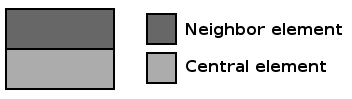
\includegraphics[width=0.7\textheight]{no_trans.png}
\end{center}
\begin{itemize}
\item equal integration order on the edge from both sides $\Rightarrow$ identical integration points
\end{itemize}
\end{frame}
\begin{frame}
\frametitle{Arbitrary-level hanging nodes with DG}
\begin{center}
1-level hanging nodes\\
use of virtual sub-elements\\
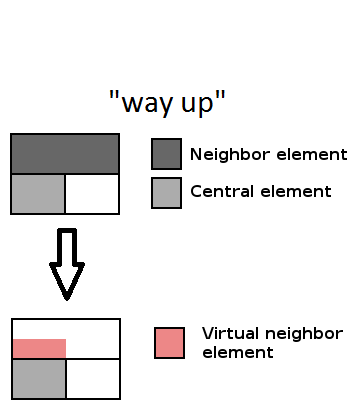
\includegraphics[width=0.5\textheight]{way_up1.png}
\hspace{4mm}
\includegraphics[width=0.75\textheight]{way_down1.png}
\end{center}
\end{frame}
\begin{frame}
\frametitle{Arbitrary-level hanging nodes with DG}
\begin{center}
2-level hanging nodes\\
use of virtual sub-elements\\
\includegraphics[width=0.45\textheight]{way_up2.png}
\hspace{4mm}
\includegraphics[width=0.8\textheight]{way_down2.png}
\end{center}
\end{frame}

%Example description
\begin{frame}
\frametitle{Model problem}
Compressible Euler equations and the advection-diffusion equation (concentration)\\\ \\
\begin{itemize}
\item
compressible Euler equations\ \\
\begin{itemize}
\item
first order system of hyperbolic laws\ \\
\end{itemize}
\item linear advection-diffusion equation
\begin{itemize}
\item second order equation
\end{itemize}
\end{itemize}
\end{frame}

%Euler equations
\begin{frame}
\frametitle{Euler equations}
Non-conservative form
\begin{eqnarray}
{\partial\rho\over\partial t} + \nabla\cdot(\rho{\bf u}) & = & 0 \\
{\partial(\rho{\bf u})\over\partial t} + \nabla\cdot(\rho{\bf u}{\bf u}^T) + \nabla p & = & 0\\
{\partial E\over\partial t} + \nabla\cdot({\bf u}(E+p)) & = & 0,
\end{eqnarray}
\begin{center}
where $E = \rho e + \frac{1}{2} \rho u^2$.
\end{center}
\end{frame}
\begin{frame}
Conservative form for DG discretization
\begin{equation}
{\partial{\bf w}\over \partial t} +{\partial{\bf f}_x\over \partial x} +{\partial{\bf f}_y\over \partial y} = 0,
\end{equation}
\vspace{-2mm}
where
\begin{eqnarray}
\nonumber
{\bf w} & = &\left(\begin{array}{c} \varrho\\ \rho u_1\\ \rho u_2\\ E \end{array} \right) 
		  = \left(\begin{array}{c} w_0 \\ w_1 \\ w_2 \\ w_3 \\ \end{array} \right)
{\bf f}_x = \left(\begin{array}{c} \rho u_1\\ \rho u_1^2 + p \\ \rho u_1 u_2\\ u_1(E+p) \end{array} \right)
			 = \left(\begin{array}{c} w_1\\ \frac{w_1^2}{w_0} + p\\ \frac{w_1w_2}{w_0}\\ \frac{w_1}{w_0}(w_3+p) \end{array} \right)\\
{\bf f}_y & = & \left(\begin{array}{c} \rho u_2\\ \rho u_2 u_1\\ \rho u_2^2 + p\\ u_2(E+p) \end{array} \right) 
			 = \left(\begin{array}{c} w_2\\ \frac{w_2w_1}{w_0}\\ \frac{w_2^2}{w_0} + p\\ \frac{w_2}{w_0}(w_3+p) \end{array} \right)\\
p         & = & {R\over c_v} \left(E-\frac{1}{2} \rho\left(u_1^2 + u_2^2\right)\right)= {R\over c_v} \left(w_3-{w_1^2+w_2^2\over{2} w_0}\right).
\end{eqnarray}
\end{frame}

%Advection-diffusion
\begin{frame}
\frametitle{Advection-diffusion equation}
\begin{eqnarray}
{\partial c \over\partial t} + \epsilon\Delta{c} + \left(\bf{u}\cdot\nabla\right) c & = & 0\\
{\partial c \over\partial t} + \epsilon\Delta{c} + \left(\frac{w_1}{w_0} \frac{\partial c}{\partial x} + \frac{w_2}{w_0} \frac{\partial c}{\partial y}\right) & = & 0.
\end{eqnarray}
Optional variational multiscale stabilization (adding a stabilization form)
\begin{equation}
S\left(u, v\right) = \int_{K} \beta \left(-\frac{w_1}{w_0} \frac{\partial v}{\partial x} - \frac{w_2}{w_0} \frac{\partial v}{\partial y} + \epsilon \Delta v\right) * \left(-\frac{w_1}{w_0} \frac{\partial u}{\partial x} - \frac{w_2}{w_0} \frac{\partial u}{\partial y} + \epsilon \Delta u\right),
\end{equation}
where
$\beta = \frac{1}{\sqrt{9 \left(\frac{4\epsilon}{|K|^2}\right)^2 + 4 \left(\frac{|u|}{|K|}\right)^2}}$ 
and $\epsilon$ is diffusivity.
\end{frame}

%Discretization
\begin{frame}
\frametitle{Discretization of time dependent problems}
\begin{itemize}
\item Rothe's method\ \\
\begin{itemize}
\item discretization in time first
\item discretized problem at each time level solved by adaptive hp-FEM
\end{itemize}
\item dynamical meshes
\begin{itemize}
\item meshes evolve in time
\item independent of each other
\\
\includegraphics[width=0.5\textheight]{shot0001.png}
\end{itemize}
\end{itemize}
\end{frame}
\begin{frame}
\frametitle{Discretization of time dependent problems}
\begin{itemize}
\item Rothe's method\ \\
\begin{itemize}
\item discretization in time first
% system of ODEs
\item discretized problem at each time level solved by adaptive hp-FEM
\end{itemize}
\item dynamical meshes
\begin{itemize}
\item meshes evolve in time
\item independent of each other
\\
\includegraphics[width=0.5\textheight]{shot0002.png}
\end{itemize}
\end{itemize}
\end{frame}
\begin{frame}
\frametitle{Discretization of time dependent problems}
\begin{itemize}
\item Rothe's method\ \\
\begin{itemize}
\item discretization in time first
% system of ODEs
\item discretized problem at each time level solved by adaptive hp-FEM
\end{itemize}
\item dynamical meshes
\begin{itemize}
\item meshes evolve in time
\item independent of each other
\\
\includegraphics[width=0.5\textheight]{shot0003.png}
\end{itemize}
\end{itemize}
\end{frame}
\begin{frame}
\frametitle{Discretization of time dependent problems}
\begin{itemize}
\item Rothe's method\ \\
\begin{itemize}
\item discretization in time first
% system of ODEs
\item discretized problem at each time level solved by adaptive hp-FEM
\end{itemize}
\item dynamical meshes
\begin{itemize}
\item meshes evolve in time
\item independent of each other
\\
\includegraphics[width=0.5\textheight]{shot0004.png}
\end{itemize}
\end{itemize}
\end{frame}
\begin{frame}
\frametitle{Discretization of time dependent problems}
\begin{itemize}
\item Rothe's	 method\ \\
\begin{itemize}
\item discretization in time first
% system of ODEs
\item discretized problem at each time level solved by adaptive hp-FEM
\end{itemize}
\item dynamical meshes
\begin{itemize}
\item meshes evolve in time
\item independent of each other
\\
\includegraphics[width=0.5\textheight]{shot0005.png}
\end{itemize}
\end{itemize}
\end{frame}

%Time discretization
\begin{frame}
\frametitle{Discretization in time}
Semi-implicit discretization\ \\
\begin{itemize}
\item linear terms discretized implicitly
\item nonlinear terms explicitly
\item possible increase of time step % with preserved stability
\end{itemize}
\end{frame}

%Space discretization
\begin{frame}
\frametitle{Discretization in space}
\begin{itemize}
\item
adaptive hp-DG for the Euler equations
\begin{itemize}
\item Steger-Warming numerical flux (easy linearization) %makes it possible to carry out the 
\item	
polynomial orders up to 10 (orders used in practice are lower)
\item
Shock capturing
\item
Flux limiting
\end{itemize}
\item
adaptive hp-FEM for the advection-diffusion equation
\begin{itemize}
\item
polynomial orders up to 10
\end{itemize}
\end{itemize}
\end{frame}


%Outputs

\begin{frame}
\frametitle{Evolution of Mach number}
\begin{center}
$$\movie[height=0.55\textheight]{\includegraphics[height=0.55\textheight]{mach.png}}{mach.avi}$$
\end{center}
\end{frame}

\begin{frame}
\frametitle{Evolution of Concentration}
\begin{center}
$$\movie[height=0.55\textheight]{\includegraphics[height=0.55\textheight]{concentration.png}}{concentration.avi}$$
\end{center}
\end{frame}


\begin{frame}
\frametitle{Comparison of meshes}
\begin{center}
Mesh for the flow (top), mesh for the concentration (bottom)\\ \animategraphics[autoplay,height=0.39\textheight]{5}{low_diff/flow_mesh/FlowMesh}{5}{5}
\\
\animategraphics[autoplay,height=0.39\textheight]{5}{low_diff/conc_mesh/ConcentrationMesh}{5}{5}
\end{center}
\end{frame}

\begin{frame}
\frametitle{Comparison of meshes}
\begin{center}
Mesh for the flow (top), mesh for the concentration (bottom)\\ \animategraphics[autoplay,height=0.39\textheight]{5}{low_diff/flow_mesh/FlowMesh}{5}{129}
\\
\animategraphics[autoplay,height=0.39\textheight]{5}{low_diff/conc_mesh/ConcentrationMesh}{5}{129}
\end{center}
\end{frame}

\begin{frame}
\frametitle{Outlook}
\begin{center}
\begin{itemize}
\item - Use the fully implicit scheme
\item - Use JFNK method (NOX package from the Trilinos library)
\item - Use the "full" Newton's method
\end{itemize}
\end{center}
\end{frame}


\begin{frame}
\frametitle{Comparison of meshes}
\begin{center}
\Large
Thank you for your attention.
\end{center}
\end{frame}


\end{document}
